\documentclass[conference]{IEEEtran}


\usepackage{graphics} % for pdf, bitmapped graphics files
\usepackage[pdftex]{graphicx}
% \graphicspath{{../pdf/}{../jpeg/}}
\usepackage{subfig}
\usepackage{xcolor}

\usepackage[cmex10]{amsmath}
\usepackage{amssymb}  % assumes amsmath package installed

\newcommand{\x}{\mathbf x}
\newcommand{\q}{\mathbf q}
\newcommand{\f}{\mathbf f}
\newcommand{\e}{\mathbf e}


\begin{document}
%%%%%%%%%%%%%%%%%%%%% TITLE %%%%%%%%%%%%%%%%%%%%%%%%%%%%%%%%%%
%\title{Image-driven robot-based drawing system itation of Human Drawing by a NAO Robot}
\title{Autonomous Motion of a Mobile Robot based on Potential Fields and Polar Control}
\author{\IEEEauthorblockN{Jose-Maria Munoz, Emanuel S. Munoz, Oscar E. Ramos}
\IEEEauthorblockA{Department of Electrical Engineering, Universidad de Ingenieria y Tecnologia - UTEC, Lima, Peru}
}
% \author{\IEEEauthorblockN{Jose-Maria Munoz\IEEEauthorrefmark{1}, Jose Avalos\IEEEauthorrefmark{1}
% Oscar E. Ramos\IEEEauthorrefmark{1}}
% \IEEEauthorblockA{\IEEEauthorrefmark{1}Department of Electrical Engineering, Universidad de Ingenieria y Tecnologia - UTEC, Lima, Peru.}
% }
\maketitle
\begin{abstract}
  Autonomous motion of mobile robots is an open problem in robotics. Challenges
  in this regard involve the proper interpretation of the information coming
  from the sensors, and the adequate motion of the robot based on that
  information to reach a goal without collisions.
%   The differential wheeled 
% robot is widely used for navigation tasks. However it has limitation in its
% motion because its non-holonomic constraints.
  In this work, we propose a framework that smoothly drives a mobile robot
  through a collision-free trajectory. The generation of trajectories is based
  on motion planning using Artificial Potential Fields and the sensed depth
  information from the environment. The generated path is then followed by an
  iterative closed-loop feedback controller based on polar coordinates which is
  guided by the potential field. With this framework the robot can autonomously
  move autonomously to a desired goal avoiding obstacles online. The framework
  continuously plans its trajectory, being able to avoid obstacles
  online. Results were obtained using a dynamic simulator and a
  differential-drive mobile robot that uses an onboard Lidar.
  % from simulations in Gazebo software for the Kobuki model and
  % from the implementation of the algorithm in real Kobuki robot sensing with a
  % Lidar sensor.
\end{abstract}
\IEEEpeerreviewmaketitle
% \textbf{\textit{Keywords - NAO Robot, Inverse Kinematics, Image Processing, Drawing Imitation}}

\section{Introduction}

Autonomy in mobile robotics is a current challenge since no flawless method for
its implementation exists. All systems have to deal with the probability of the
sensors and with the proper interpretation of the information. In spite of
these problems, mobile robots are widely used in applications such as
exploration and navigation on the ground \cite{Bonin-Font2008}.  One
particularly useful type of mobile robot is the differential wheeled robot
since its dynamics and physical structure is not complex. However, its motion
has to deal with their inherent non-holonomic constraints \cite{Rubayat}.
%application in navigation of these robots deals with some problems for the controllability of its kinematics.
%The robot is a non-holonomic system, so the controllability of these robots is difficult to achieve.
These constraints need to be taken into account when doing trajectory tracking
in any environment since the control needs to be done at the velocity level
rather than at the position level.
% For example, the robot cannot smoothly achieve a goal because its orientation
% is significantly important to its motion.
% Some approaches to this solution has gone through different approaches \cite{Rubayat}. 
% In general, these approaches can be divided for the model in a different system of coordinates.
The usage of polar coordinates facilitates the control of the robot in a
Cartesian coordinate system, and control laws based on these coordinates have
the potential to smoothly achieve exponential stability through closed-loop
control \cite{Matoui}. However, the mathematical formulations of these control
laws do not consider trajectory constraints, and a higher level system must
guide the motion when autonomy is to be reached.
% Moreover, polar control laws can
% be used for obstacle avoidance when used with appropriate frameworks and a
% higher level system must guide the motion when autonomy is to be reached. 
% if there are obstacles if it is stated middle goals in which the robot can avoid them. However, these middle goals must be formulated arbitrarily, which is not a good approach for the autonomy of the robot in a navigation task.

Practical applications of mobile robots deal with real environments where, by
nature, several obstacles exist. Therefore, it is necessary to avoid these
obstacles when moving. There exist different approaches for solving the path
planning problem. One of them is the artificial potential field (APF)
\cite{Woods}. However, for non-holonomic robots, the path generated using it
can be hard to follow through conventional control methods such as a classic
PID controller because of the non-holonomic constraints imposed by the
mechanical structure.
%or the two-wheeled robot, its non-holonomic problem impede a normal path planning through this method. The artificial attractive or repulsive forces formulate trajectories which the robot cannot follow through conventional control methods. 

In this work, we propose an autonomous motion framework based on potential
fields and on polar control laws for the motion of a mobile robot so that it is
able to reach a goal continuously replaning its path without collisions. Our
framework is able to work online and onboard. Experimental results were
obtained through the implementation of each individual controller in a
differential drive robot using a dynamic simulator. Then, the approach was also
tested on a real Kobuki robot powered with a Lidar sensor as shown in
Fig.~\ref{fig:example-robot}. The onboard controller of this robot was done
using a Raspberri Pi3 computer, which allowed the robot to achieve autonomy.
% Posteriorly, the integration of the controllers for obtaining the proposed control is implemented in a real Kobuki robot powered with a Lidar sensor for obtainment of position obstacles. 
% This work is structured as follows. In section \ref{sec:robot_motion}, it is introduced the forward and inverse kinematics. Section  \ref{sec:APF} formulates the potential field equation for its application as well as it is stated the control laws in the polar coordinate system.Finally, the experimental results and conclusion are shown to give details of the implementation.

\begin{figure}%[h]
  \centering \footnotesize
  \subfloat
  {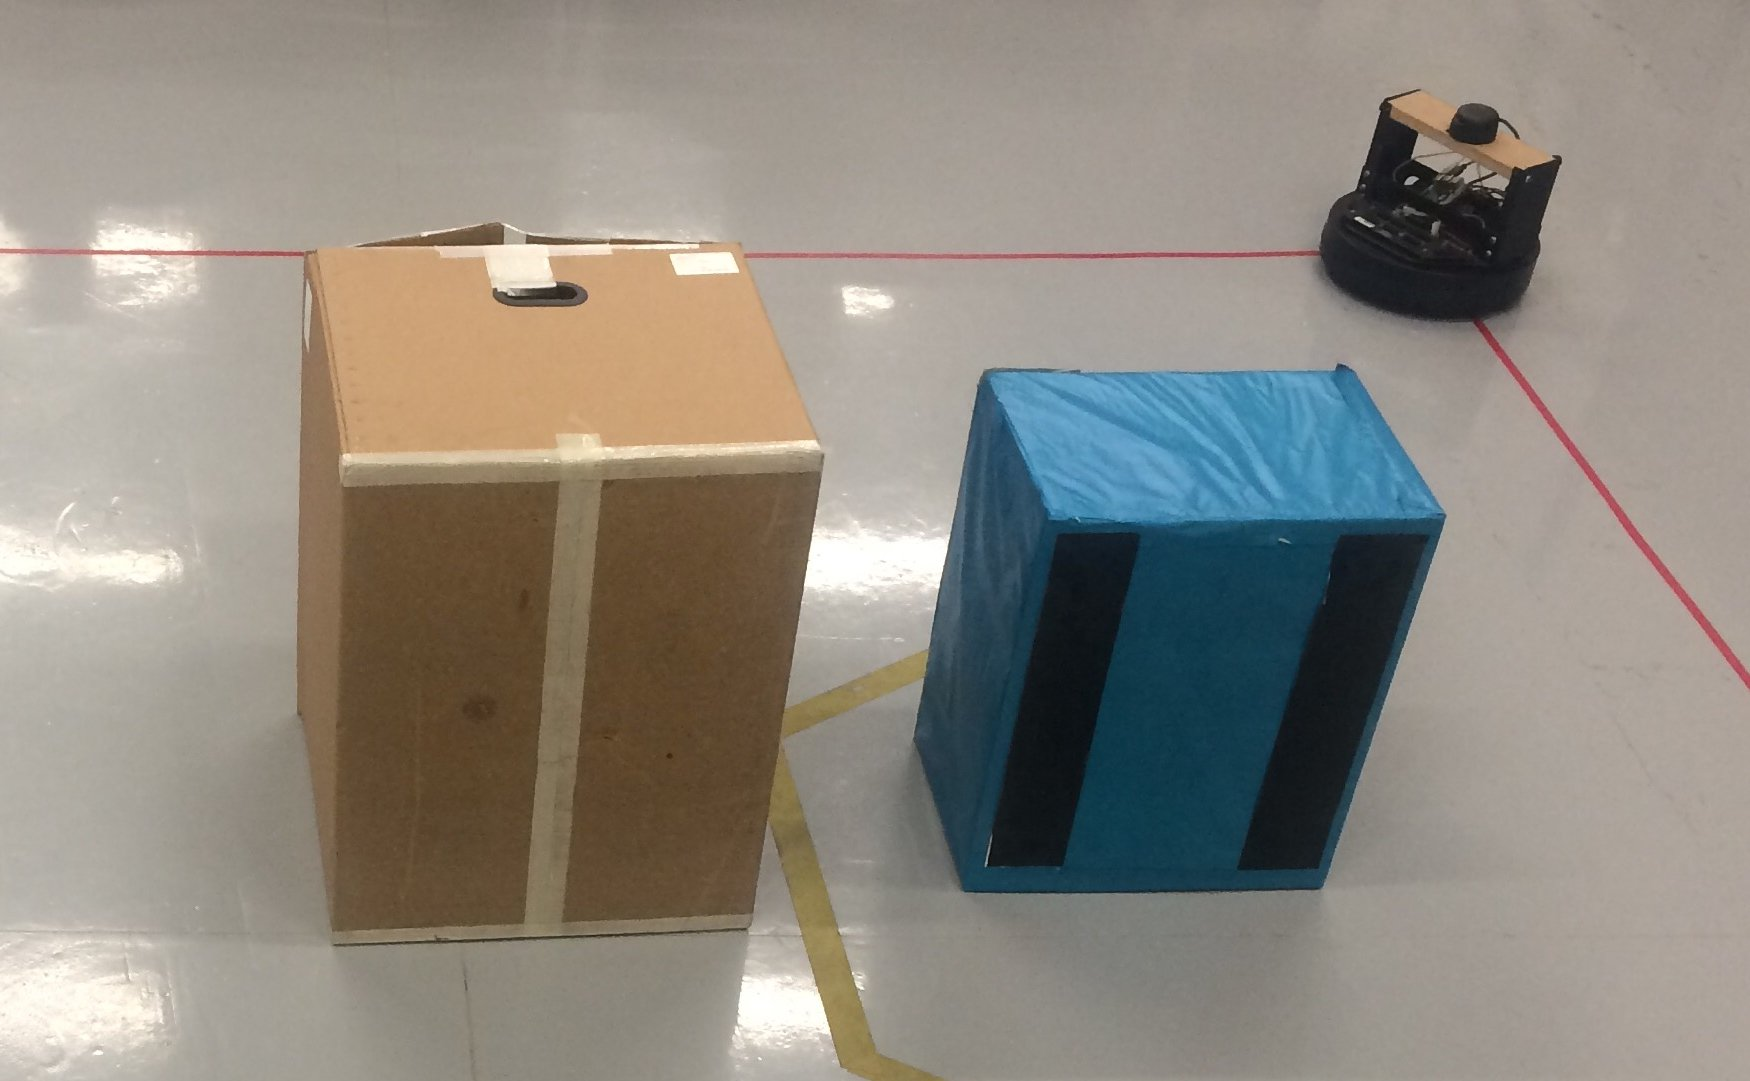
\includegraphics[width=0.4\textwidth]{kobuki}}
  \captionsetup{font=footnotesize}
  \caption{Experimental setup for testing the autonomy of the mobile robot. A
    goal position is given behind the obstacles so that the robot cannot follow
    a straight line but needs to autonomously determine its right path online.}
  \label{fig:example-robot}
\end{figure}


\section{Framework for Robot Autonomy}

\subsection{Robot Motion Control}
\label{sec:robot_motion}

The first step towards achieving an autonomous robot is to generate proper
motion through an adequate controller. To this end first the kinematic model
that relates the velocity of the wheels to the linear and angular velocity of
the robot in its own reference frame needs to be computed. This is a well-known
problem and assumes that each wheel of the robot has a low-level velocity
controller. After computing the kinematics, it has to be properly used to drive
the robot motion. One classical way is to use a standard PID (Proportional,
Derivative, Integral) controller that considers the 2D error in Cartesian
space. Although a PID controller is suitable for several processes, it is
usually not a very good choice when dealing with mobile robots, specially those
that have non-holonomic constraints such as differential drive robots.

% For navigation in a wheeled differential robot, it is necessary to control its motion appropriately. A classic way is using a PID controller in the Cartesian space. However, this control is usually ill-posed for a differential wheeled robot.
%In this section, the kinematics of the robot is recalled, and the control laws for its motion based on a polar approach is presented.
% In this section the control laws for its motion based on a polar approach is presented.
%\subsection{Polar controller}
An alternative way to achieve a softer motion in position and orientation is to
use the so-called \textit{polar controller}, which provides a linear control
law using feedback of the states and a description inspired by polar
coordinates. As Fig.~\ref{fig:Polar} shows, the polar coordinates associated
with the robot are
\begin{align*}
  \rho &= \sqrt[]{(x_{d} - x)^2 + (y_{d} - y)^2}  \\
  \alpha &= \text{atan2}(y_{d} - y, x_{d} - x) - \theta  \\
  \beta &= -\text{atan2}(y_{d} - y, x_{d} - x) + \theta_{d}.
\end{align*}
where $\rho$ represents the distance from the robot to the goal position,
$\alpha$ and $\beta$ are angles that are used for the error in orientation. The
current pose of the robot is $\x=(x,y,\theta)$, and its desired pose is
$(x_d,y_d,\theta_d)$. 
\begin{figure}%[h]
 \centering \footnotesize
  \subfloat
  {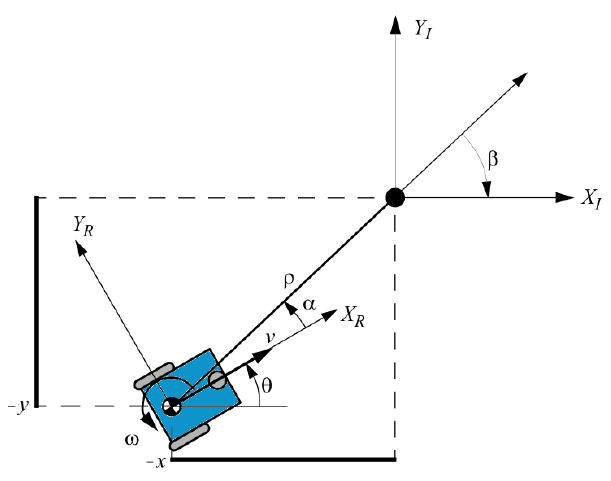
\includegraphics[width=0.7\linewidth]{control_polar.png}}
  \captionsetup{font=footnotesize}
 \caption{Setup for the polar control where the current position of the robot
   as well as the goal position and specific parameters are shown.}
 \label{fig:Polar}
\end{figure}
Based on these polar variables, the control law that defines the linear and
angular velocities so as to achieve the desired pose is
\begin{align}
  \label{eq:v}
  v &= k_{\rho}\rho \\
  \label{eq:w}
  \omega &= k_{\alpha}\alpha + k_{\beta}\beta
\end{align}
where $k_{\rho}$, $k_{\alpha}$, and $k_{\beta}$ are the polar controller gains
that need to be properly tuned for a good response of the system. Using this
motion generation framework we achieve the goal both in position and in
orientation.


\subsection{Path Generation through Potential fields}
\label{sec:APF}

Once the motion has been properly controlled, it is necessary to determine the
path that the robot should track. We use an artificial potential scheme in this
work to autonomously generate this path online based on the data obtained from
the onboard sensor.
% \subsection{Artificial Potential Field}
% There exist several approaches in path planning through potential field. In
% this case, we opted for a one which considers some assumptions for its
% implementation.
A potential field generates a force field that drives the robot towards the goal
avoiding obstaces. This force has two components, an attractive potential field
and a repulsive potential field.

\subsubsection{Attractive Potential Field}

This field drives the robot towards the goal position assuming that there is a
certain ball around this goal. That is, any position inside this ball will be
considered as satisfying the objective of the planning algorithm. Consider a
scalar potential energy which depends on the distance between the current
position of the robot $q=(x,y)$, and its goal position
$q_{goal}=(x_{goal},y_{goal})$ as
\begin{equation}
	U_{att}(q) = \frac{1}{2} \zeta d^2(q,q_{goal})
	\label{eq:pot_attr}
\end{equation}
where $d(a,b)$ is some metric measurement between two points, and $\zeta$ is a
tuning parameter that scales the effect of the attractive potential. In this
case, we used the Euclidean distance as a metric since it provides good
experimental results. The gradient of this field provides a vector field which
always points to the desired goal position as:
\begin{equation}
  \label{gradient_att}
    \nabla U_{att}(q)= \zeta(q - q_{goal}).
  % \begin{aligned}
    % \nabla U_{att}(q) &= \nabla (\frac{1}{2}\zeta d^2 (q,q_{goal})),\\
    % &=\frac{1}{2}\zeta \nabla d^2(q,q_{goal})\\
    % &= \zeta(q - q_{goal})
  % \end{aligned}
\end{equation}

The resulting vector points away from the goal with magnitude $\zeta$ at all
points of the configuration space, except at the goal where it is
undefined. Starting from any point other than the goal, and following the
negated gradient, a path is traced towards the goal.
% The equation \ref{gradient_att} is a vector based at $q$, points away from $q_{goal}$, and has a magnitude proportional to the distance from $q$ to $q_{goal}$.\\

\subsubsection{Repulsive Potential Field}

A repulsive potential keeps the robot away from obstacles. The strength of the
repulsive force depends upon the robot's proximity to the obstacle. The closer
the robot is to an obstacle, the stronger the repulsive force should
be. Therefore, the repulsive potential is usually defined in terms of distance
to the closest obstacle $D(q)$ as 
\begin{equation}
  U_{rep}(q) = 
  \begin{cases}
    \frac{1}{2}\eta(\frac{1}{D(q)} - \frac{1}{Q*})^2, & D(q)\leq Q^* \\
    0, & D(q) > Q^*
  \end{cases}
  \label{eq:pot_rep}
\end{equation}
where $Q^* \in \mathbb R$ is a constant that allows the robot to ignore
obstacles that are sufficiently far away from it, and the $\eta$ is a gain on
the repulsive gradient. The gradient is
\begin{equation}
  \nabla U_{rep}(q) = 
  \begin{cases}
    \eta (\frac{1}{Q^*} - \frac{1}{D})\frac{1}{D^2} \nabla D, &D \leq Q^*\\
    0 , &D > Q^*
    % \eta (\frac{1}{Q^*} - \frac{1}{D(q)})\frac{1}{D(q)^2} \nabla D(q), &D(q)
    % \leq Q^*\\
    % 0 , &D(q) > Q^*
  \end{cases}
  \label{eq:force_rep}
\end{equation}
where the dependency of $D$ on $q$ has been omitted for clarity. The scalars
used for this field are usually determined by trial and error.

\subsection{Algorithm for Autonomous Motion}
\label{sec:algor}
To make the robot move to its final goal without bumping into obstacles, the
following approach was taken. First, a desired final goal
$q_g=(x_g, y_g, \theta_g)$ that describes the position and orientation is
specified in terms of the inertial frame. Then, the current local environmental
data is obtained from a sensor such as a Lidar, which we used in the
experiments, but any other depth sensor can be used. These data provides the
positions of the obstacles that are in the field of view of the robot, and they
are used as obstacle positions that define the repulsive field.

Using the potential field defined by the goal and the sensed data, a step in
the direction of the total field at the current position is taken. This step
uses a small increment in this direction and defines the desired pose that the
polar controller must follow. As the robot moves, this desired pose also
changes according to the potential field, guiding the motion towards the goal
and avoiding the obstacles. Note that as the robot moves it continues scanning
and updating its obstacle map and thus, updating the whole potential field
composed of the attractive and repulsive parts.  

% it is posteriorly used a guide to generate middle-goals for the polar control. In that way, it is only necessary the positions of the robot, the goal and the obstacles, so it could be generated a vector field from the sum of the attractive  and repulsive potential field.\\

\section{Results}

The proposed methodology was tested on a real Kobuki mobile robot, which is a
differential drive robot, and an RP Lidar attached to it. The interface between
both elements was done using a Raspberri Pi3 running ROS (\textit{Robot
  Operating System}). Using this framework, it is also possible to online
stream the acquired data to an offboard computer.

\subsection{Modular Experiments}

% The potential field approach was implemented to perform different tasks in
% different situations and thus have a robust behavior. This algorithm works with
% forces of atrraccion and repulsion. The first is used to reach the desired
% position and the second force is to avoid obstacles.
The forces provided by the artificial potential field were decomposed in
magnitude and direction that continuously drive the robot. To show how the
approach works, an offline test that uses artificially located goals and an
obstacle was performed. Figure \ref{f:apf}(a) shows the attraction field and
the forces that guide towards the obstacle. The simulated robot is initially
located at the top left corner $q_0=(2,18)$ and it moves towards the goal
$q_{goal}=(10,4)$ guided by the field. The white points show the followed path
that the robot should follow, and which will later guide the controller. A pure
repulsive field is shown in \ref{f:apf}(b), where three obstacles in different
positions of the workspace were added. Each obstacle is projected as a red
circle due to its high magnitude within its potential field, where the forces
point outward in each obstacle. The total navigation force composed of the
superposition of the attraction and repulsive forces is shown in Figure
\ref{f:apf}(c).
% , where the white points is the trajectory that the robot would
% generate assuming that this robot has a controller that overcomes
% non-holonomicity without having restrictions for its movement.

% To check the
% efficiency of the algorithm, it was simulated graphically in a workspace where
% the vector field was projected, indicating the potential field algorithm forces
% for different positions of the obstacles and the desired position.The forces of
% atrraccion can be observed in Figure \ref{f:apf}(a), where the desired position
% is $ (10,4) $ and the initial position of the robot is $ (2,18) $. The white
% points within the image refer to the desired semi-positions forming the path of
% the robot. You can also see that all the arrows in the vector field are in the
% direction of the robot's goal. Likewise, also in Figure \ref{f:apf}(b) you can
% see three obstacles that are distributed in different positions of the
% workspace. Each obstacle is projected as a red circle due to its high magnitude
% within its potential field, where the forces point outward in each
% obstacle. Finally, for the force of navigation, the forces of attraction and
% repulsion had to be superimposed, as shown in Figure \ref{f:apf}(c). Where the
% white points is the trajectory that the robot would generate assuming that this
% robot has a controller that overcomes non-holonomicity without having
% restrictions for its movement.


%Potential field fue implementado para que pueda realizar diferentes tareas en diversas situaciones y así tener un comportamiento robusto. Este algoritmo trabaja con fuerzas de atrraccion y repulsion. El primero es utilizado para llegar a la posicion deseada y la segunda fuerza es para evitar obstaculos. Estas fuerzas fueron descompuestas en magnitud y direccion para que el robot pueda tomar semi posiciones deseadas para cada iteracion.
%Para comprobar la eficiencia del algoritmo se simulo de forma gráfica en un espacio de trabajo donde se proyectó el campo vectorial indicando las fuerzas del algoritmo potential field para diferentes posiciones de los obstaculos y de la posicion deseada. 
%Las fuerzas de atrraccion se pueden observar en la Figura \ref{f:apf}(a), donde la posición deseada es $(10,4)$ y la posicion inicial del robot es $(2,18)$. Los puntos de color blanco dentro de la imagen hacen referencia a las semi posiciones deseadas formando la trayectoria del robot. Tambien se puede ver que todas las flechas,del campo vectorial,estan en direccion hacia la meta del robot. Asimismo, también en la Figura \ref{f:apf}(b) se puede observar a tres obstaculos que estan distribuidos en diferentes posiciones del espacio de trabajo. Cada obstaculo se proyecta como un circulo rojo debido a su alta magnitud dentro de su campo potencial, donde las fuerzas apuntan hacia afuera en cada obstaculo. Finalmente, para la fuerza de navegacion se tuvo que superponer las fuerzas de atraccion y repulsion como se observa en la Figura \ref{f:apf}(c). Donde los puntos blancos es la trayectoria que generaría el robot asumiendo que este robot tiene un controlador que supera la no holonomicidad no teniendo restricciones para su movimiento.

% \begin{figure}%[ht!]
%   \centering
%   \subfloat[Attractive Force]{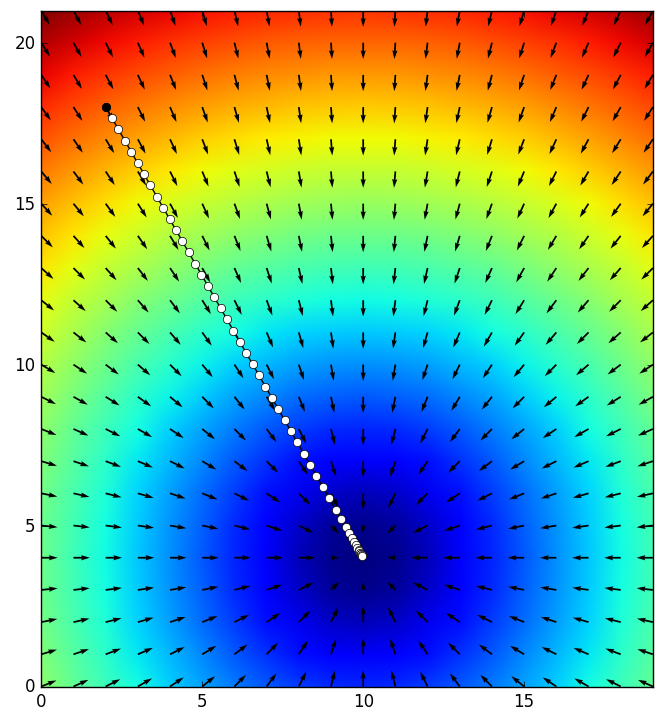
\includegraphics[width=40mm]{attr_force2.png}}
%   ~\subfloat[Repulsive Force]{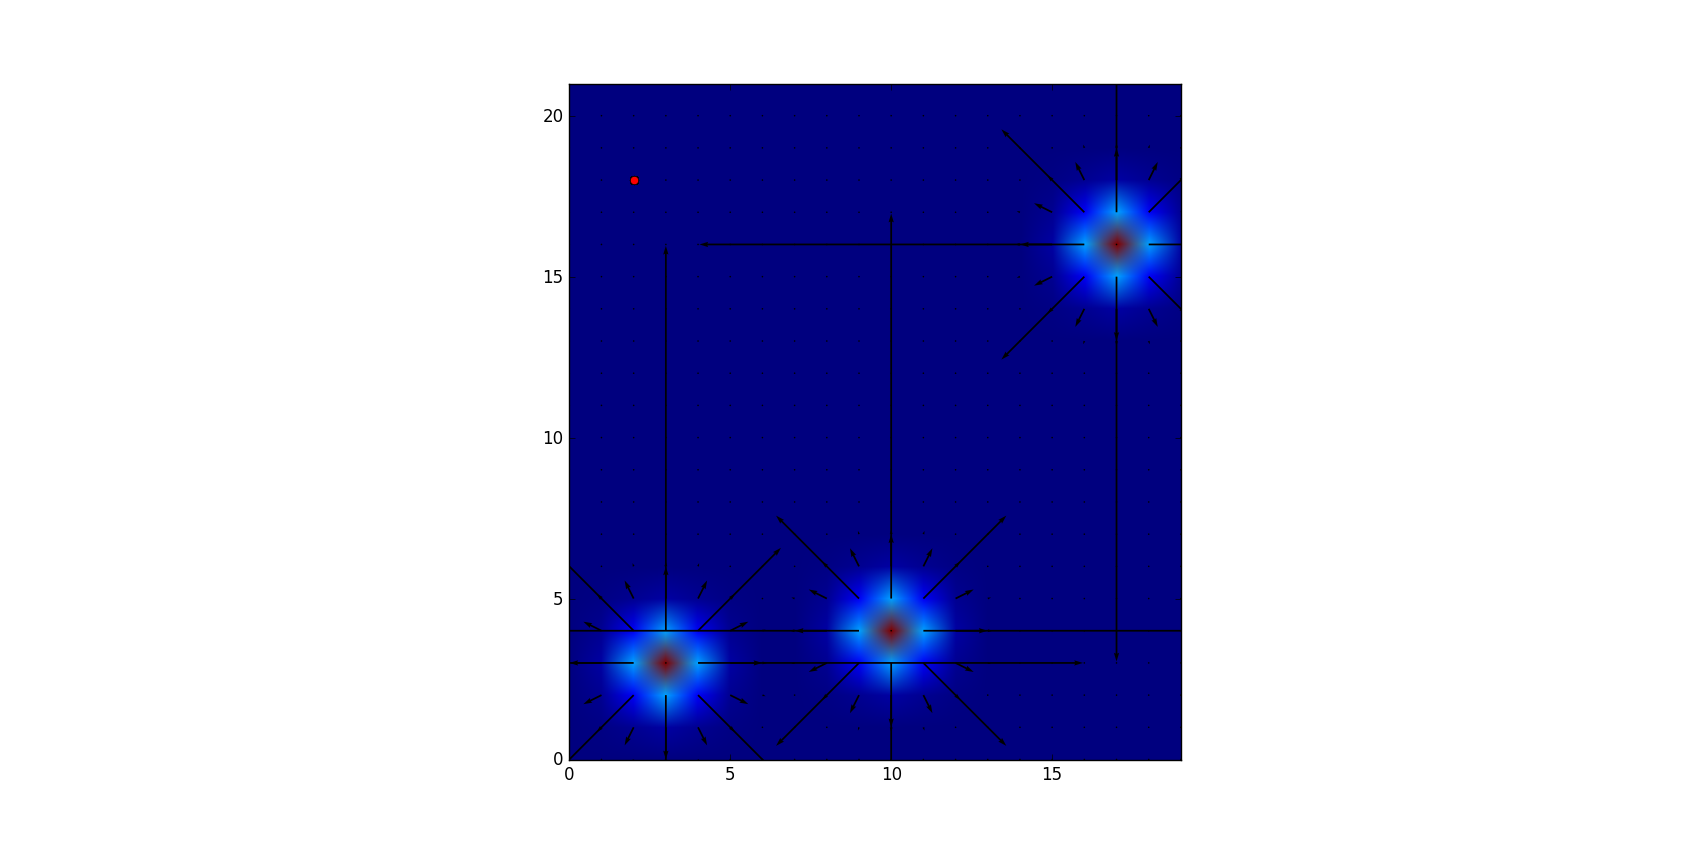
\includegraphics[width=40mm]{rep_force.png}}\\
%   \subfloat[Navigation Force]{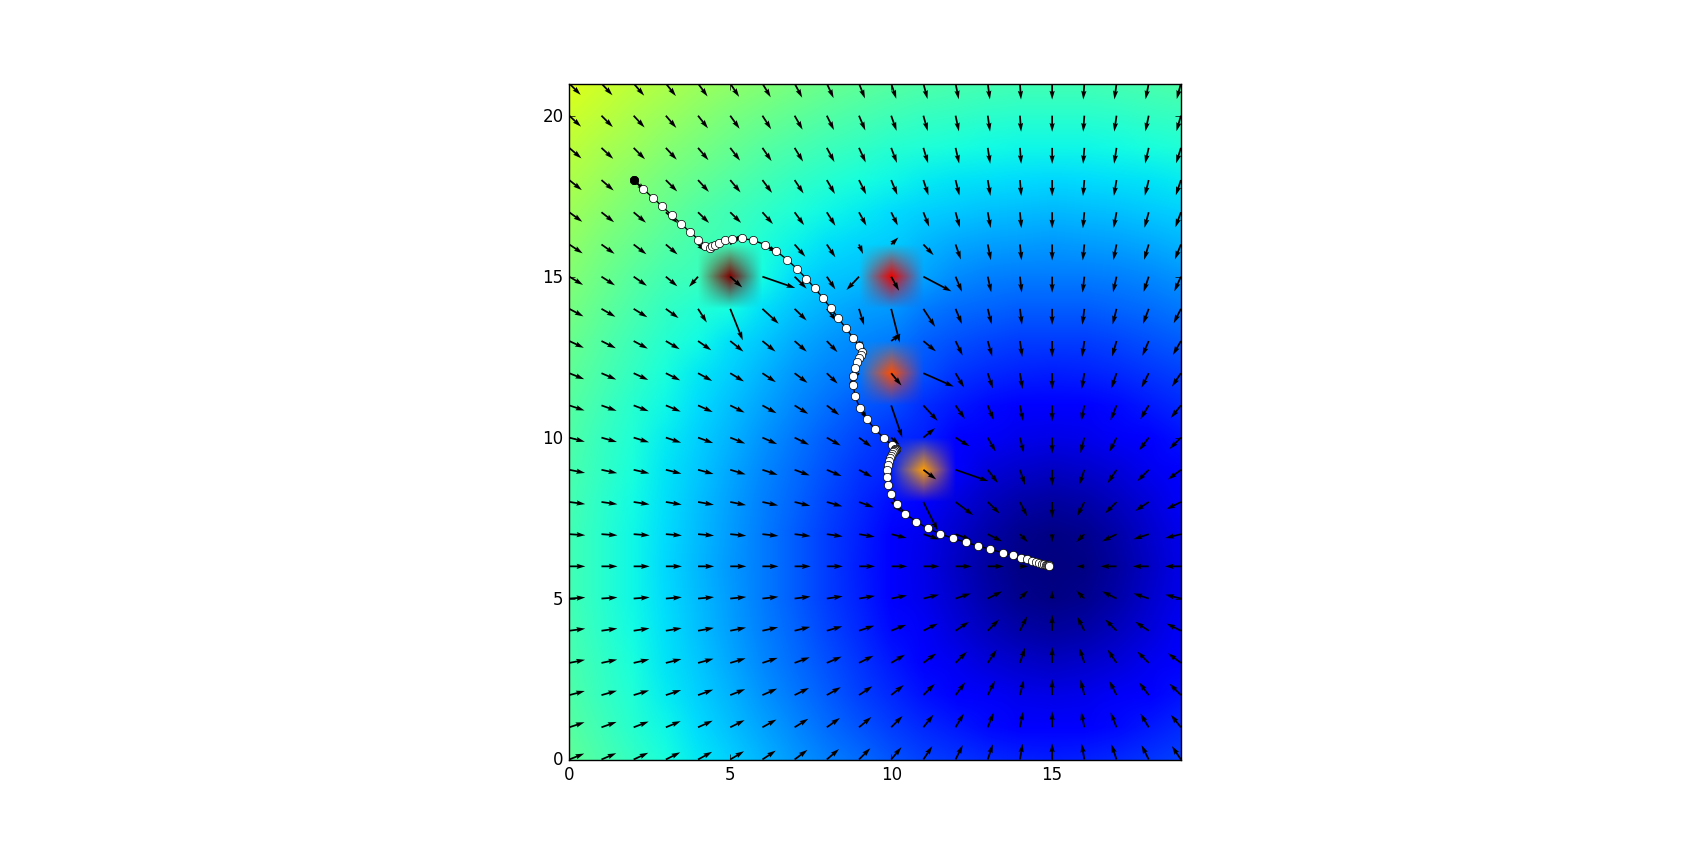
\includegraphics[width=40mm]{nav_force.png}}
% %\subfloat[Attractive Force]{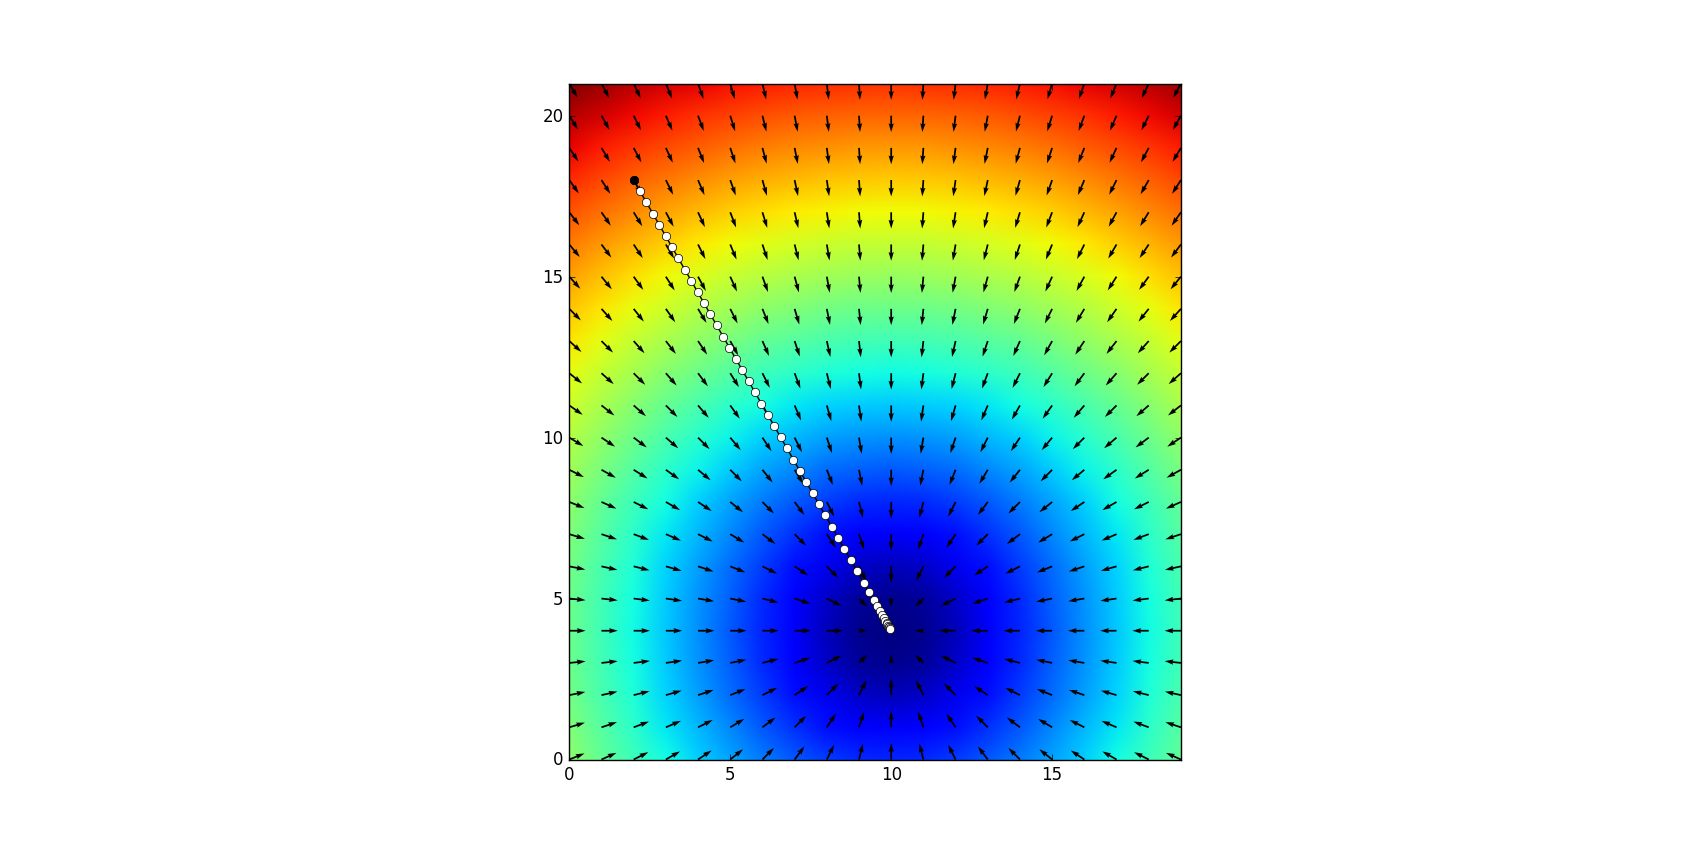
\includegraphics[width = 150mm]{attr_force.png}}
%   \caption{Potential Field Algorithm} \label{f:apf}
% \end{figure}

\begin{figure}%[ht!]
  \centering \footnotesize
  \subfloat[Attractive Force]{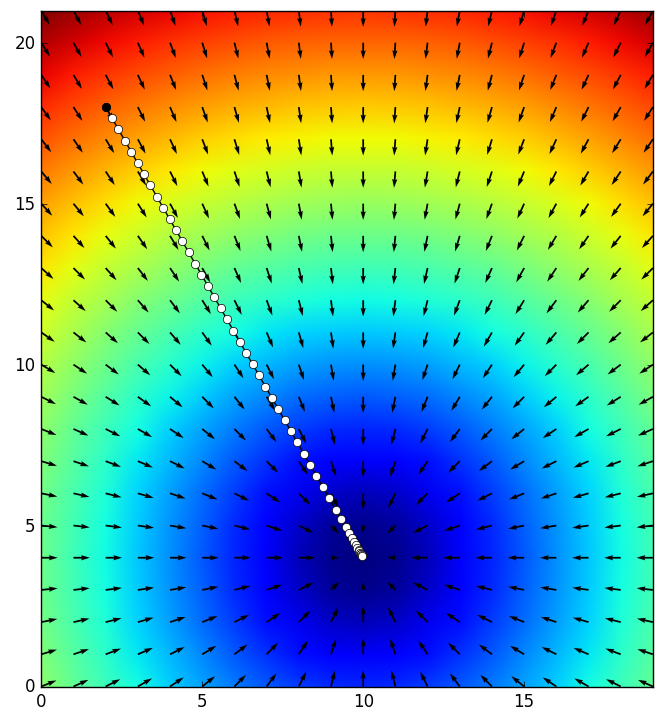
\includegraphics[width=0.16\textwidth]{attr_force2.png}}
  ~\subfloat[Repulsive Force]{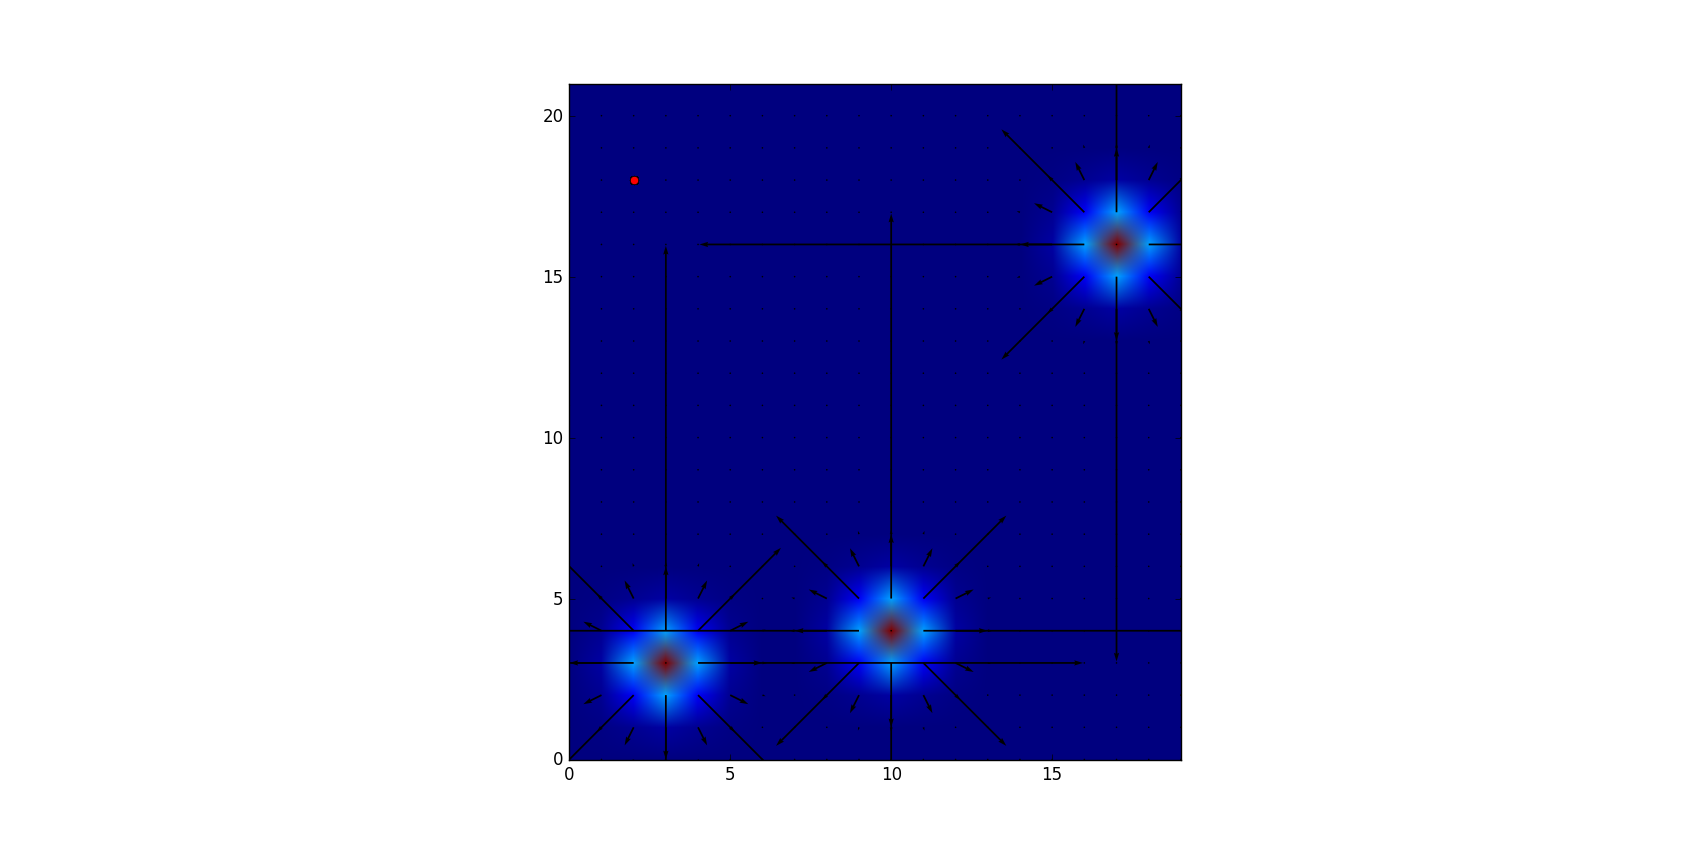
\includegraphics[width=0.16\textwidth]{rep_force.png}} ~
  \subfloat[Navigation Force]{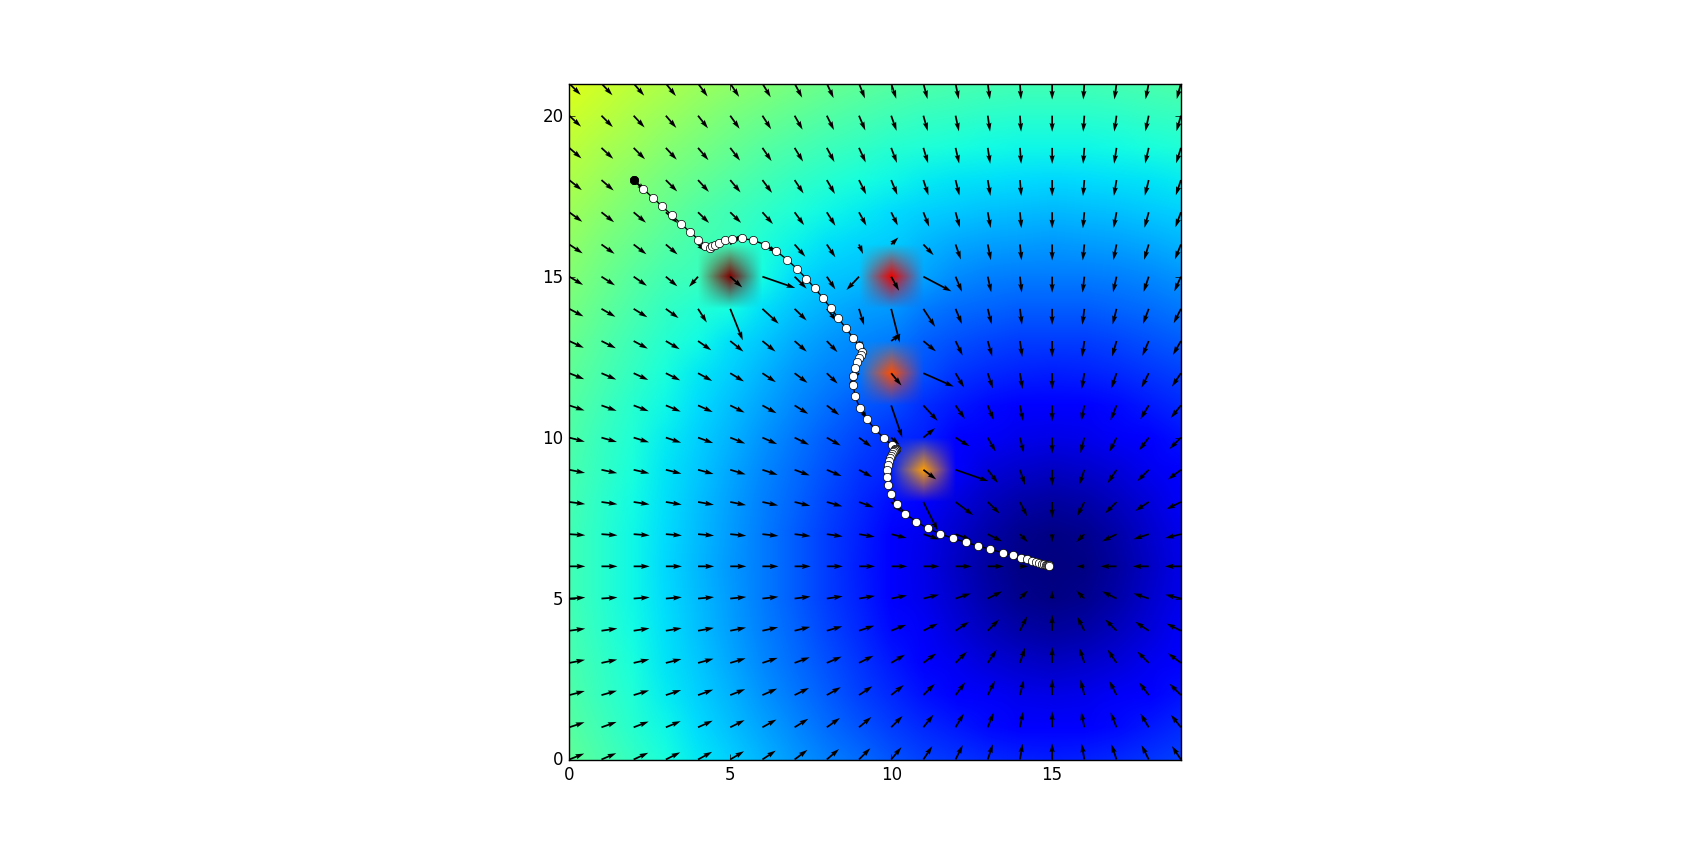
\includegraphics[width=0.16\textwidth]{nav_force.png}}
  % \subfloat[Attractive Force]{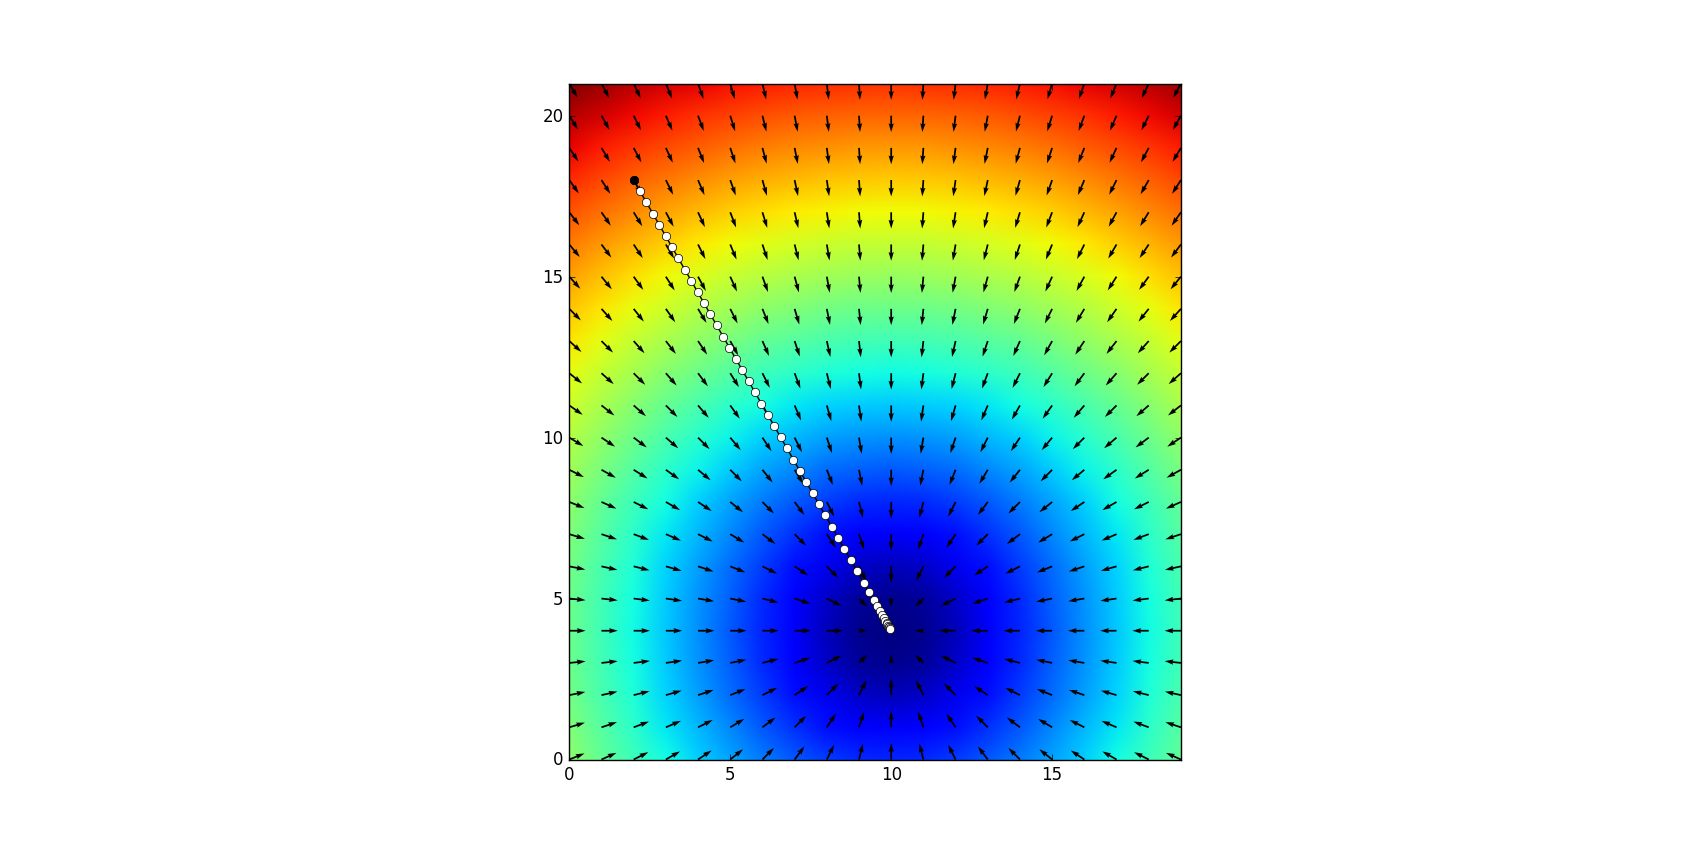
\includegraphics[width = 150mm]{attr_force.png}}
  \captionsetup{font=footnotesize}
  \caption{Tests for the Potential Field Algorithm} \label{f:apf}
\end{figure}

% \subsection{Polar controller}

To test the polar controller, a dynamic simulation was used in Gazebo with the
Kobuki robot and without obstacles, and the state variables including velocity,
position, and orientation were obtained online from the simulated odometry.
% The objective of the tests was to move the
% robot to a given random goal pose. % It was considered a start position in the
% origin of the frame and the desired position ($x,y,\theta$) respect to the same
% inertial frame. 
% The state variables (velocity, position and orientation) of the robot were
% obtained from the simulated odometry and the controller was applied online.
Using the feedback from this odometry, the controller was applied online. For
these tests, the goal position was
($x = 3,y = 3$), and the goal orientation $\theta = 90^{\circ}$.
% The start time of simulation
% is approximately 7 seconds because of a delay of the software.
% For every figure, the variation of the variable is immediate and in a
% homogeneous convergence time.
Figure \ref{f:polar}(a) shows the temporal
evolution of the position ($x$) where a convergence to the desired position is
achieved in less than 20 seconds. This is due to the distance to the
obstacle. Different distances lead to different convergence times, and the
convergence rate can also be modified changing the gains in \eqref{eq:w} for
the angular velocity, and in \eqref{eq:v} for the linear velocity. The other
sublots in Fig.~\ref{f:polar} show the temporal evolution of the linear
velocity in $x$, the orientation and the angular velocity.
% , there is a peak in the curve which diverges from the goal orientation.
For orientation, there is an overshoot which is due to the over-dependence of
the controller on position instead of orientation.
% This characteristic is
% mainly upward for a navigation resolution.


% The polar controller was implemented for the Kobuki motion in a virtual workspace in Gazebo with no obstacles. The prompt of the proofs was the robot to achieve a given a random goal position.  It was considered a start position in the origin of the frame and the desired position ($x,y,\theta$) respect to the same inertial frame. The state variables (velocity, position and orientation) of the robot was obtained from odometry. The performance of the robot for one of the experimental cases is shown in the following figures.

% The graphical results show the performance of the robot for a goal position ($x = 3,y = 3$) and orientation ($\theta = 90°$). The start time of simulation is approximately 7 seconds because of a delay of the software. For every figure, the variation of the variable is immediate and in a homogeneous convergence time. In contrast, the Figure \ref{f:polar}(a) shows a rapid convergence of the position compared to the other variables. In the same way, in Figure \ref{f:polar}(c), there is a peak in the curve which diverges from the goal orientation. These results proves an over-dependence of the controller to the position instead of the orientation. This characteristic is mainly upward for a navigation resolution.


\begin{figure}
  \centering
  \subfloat[Position (x) evolution]{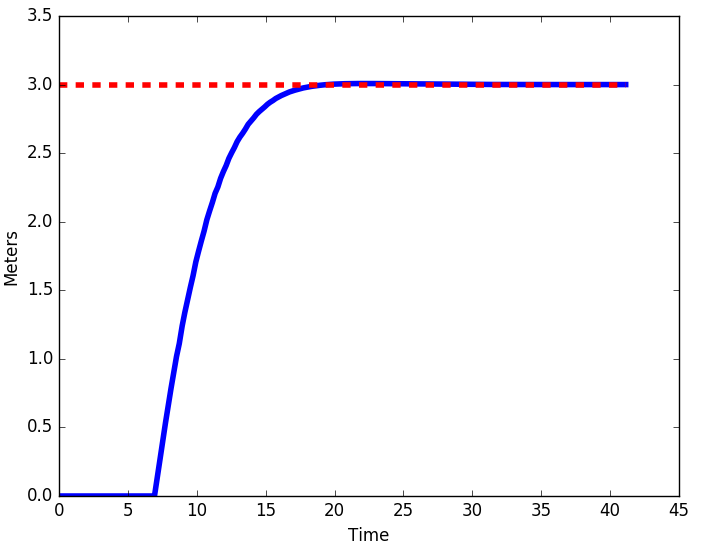
\includegraphics[width = 40mm]{tvsxy_tesis.png}}
  ~\subfloat[Linear velocity evolution]{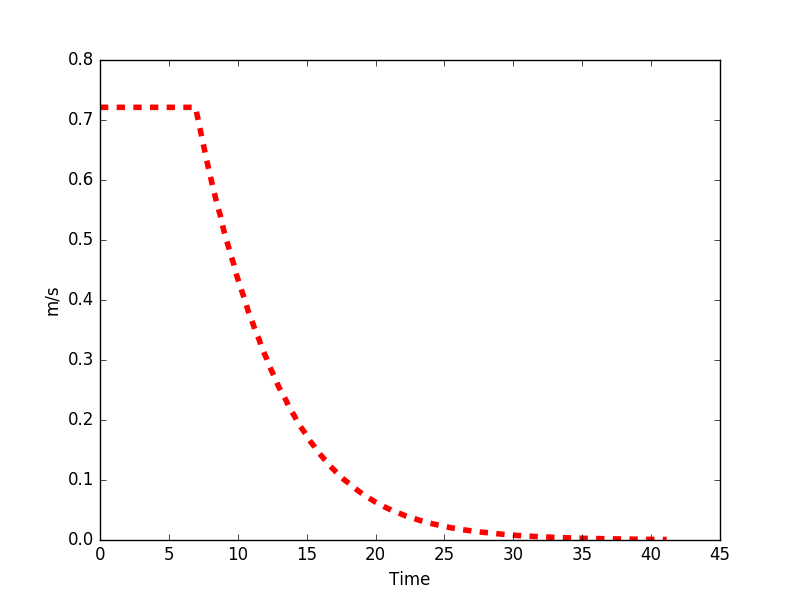
\includegraphics[width = 40mm]{tvsv_tesis.png}}\\
  \subfloat[Orientation evolution]{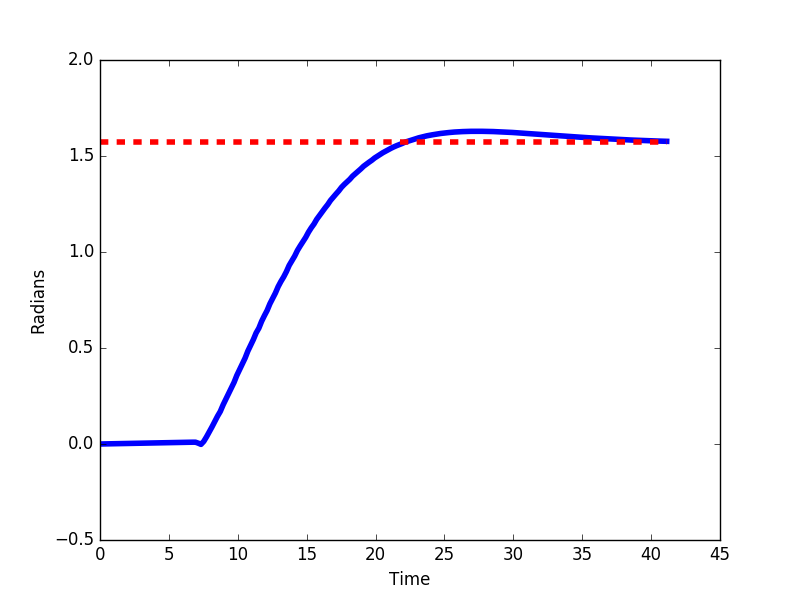
\includegraphics[width = 40mm]{tvstheta_tesis.png}}
  ~\subfloat[Angular velocity evolution]{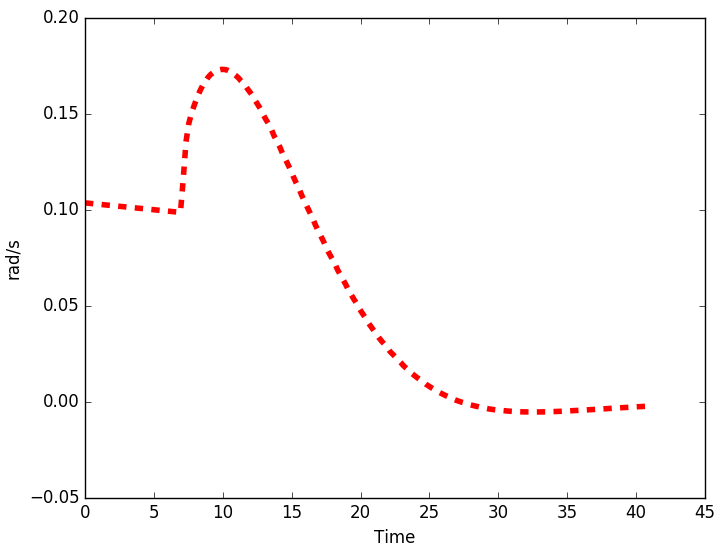
\includegraphics[width =
    40mm]{tvsomega_tesis.png}}
  \captionsetup{font=footnotesize}
  \caption{Temporal evolution of the state variables using a polar controller
    to achieve a desired position given by $x=3, y=3, \theta=90°$} \label{f:polar}
\end{figure}

\subsection{Autonomous Navigation}

The proposed framework was implemented as an iterative algorithm in the Kobuki
robot. As described in section~\ref{sec:algor}, the algorithm iteratively takes
middle goal positions through the artificial potential field and the polar
controller drives the robot across them. We exposed the robot to different
obstacles whose positions were a priori known.
% The performance of the robot is shown in the following figures:
Fig.~\ref{f:kbki}(a) shows the the attractive forces for every position (red
dots) in which the algorithm is iterated in the two-dimensional environment
within the robot motion. For every position, the attractive potential field
drives the robot to the goal position which is verified by the arrows.
% Note that this trajectory is not sent to the robot since it didntThe
% trajectory shown in this figure is not forward to the goal because of the
% obstacles, which are not considered for the attractive APF.  Figure
Fig~\ref{f:kbki}(b) is composed of the repulsive forces based on the obstacles,
which are shown as green markers.
% The forces are only applied, as it was
% formulated above, for less than a arbitrarily range (for this result it was
% considered 1 meter). For each obstacle, the magnitude of the forces increases
% as long as the robot is closer to it. Also, its direction points toward to the
% position of the robot, so it bring an opposite force to the attractive
% potential field.  Figure \ref{f:kbki}(c) shows the superposition of the forces
% with the actual obstacles. Each forces provides a middle goal position for the
% robot, thus it is the input variable for the polar controller. Even though the
% forces close to the obstacles have a high rate of change, the trajectory is
% smooth. It demonstrates the effectiveness of the polar controller despite its
% non-holonomic charateristic.
For each obstacle, the magnitude of the forces increases when the robot is
closer to it, and their direction points out of the obstacles, allowing the
robot to avoid them. Fig.~\ref{f:kbki}(c) shows the superposition of both
forces with the real obstacles. Each forces provides an intermediate goal
position for the robot, constituting the continuously updated desired pose for
the polar controller. Even though forces close to the obstacles have a high
rate of change, the trajectory is smooth. This demonstrates the effectiveness of
the polar controller despite the non-holonomic characteristics of the robot.
% \begin{figure}
%   \centering
%   \subfloat[Attractive force applied to the mobile robot]{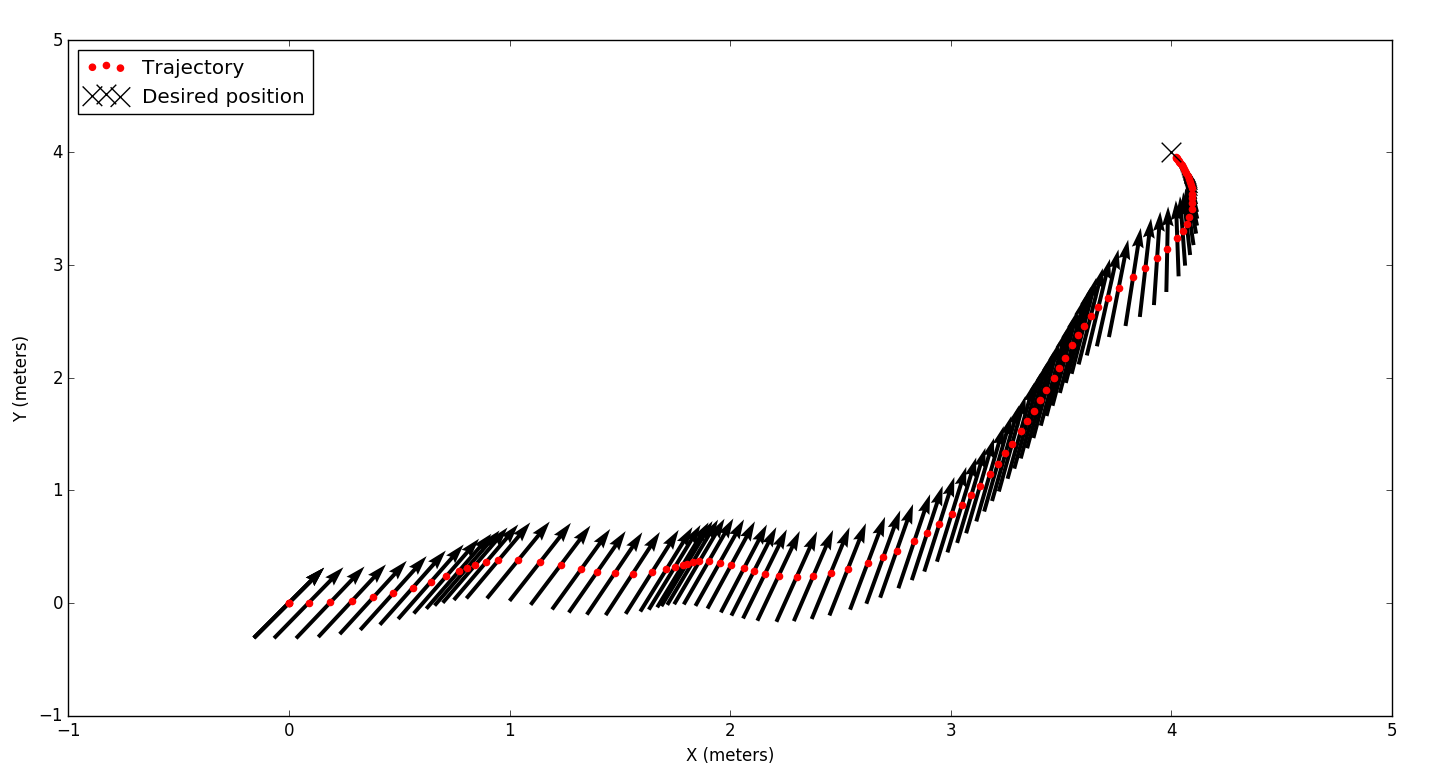
\includegraphics[width = 65mm]{attr_kbki.png}}\\
%   \subfloat[Repulsive force applied to the mobile robot] {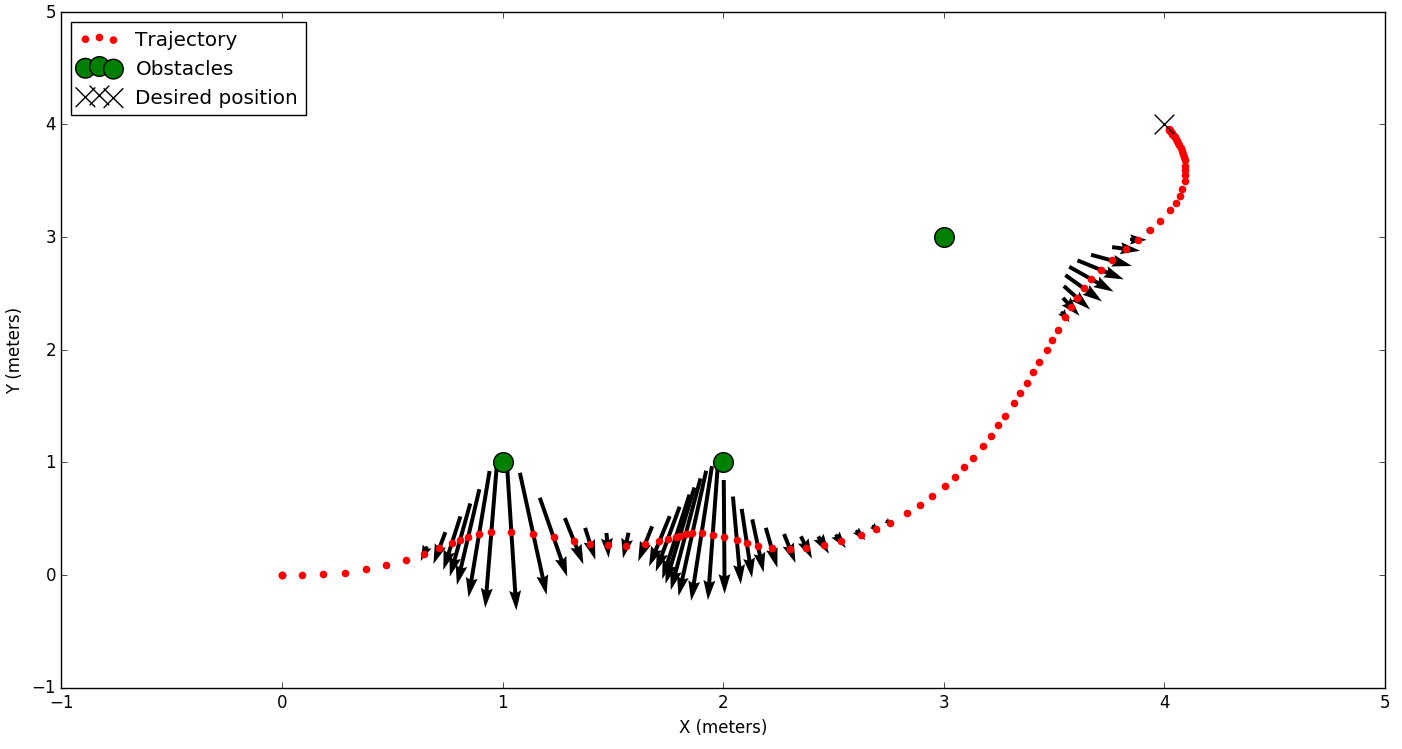
\includegraphics[width = 65mm]{rep_kbki.png}}\\
%   \subfloat[Navigation force applied to the mobile robot]{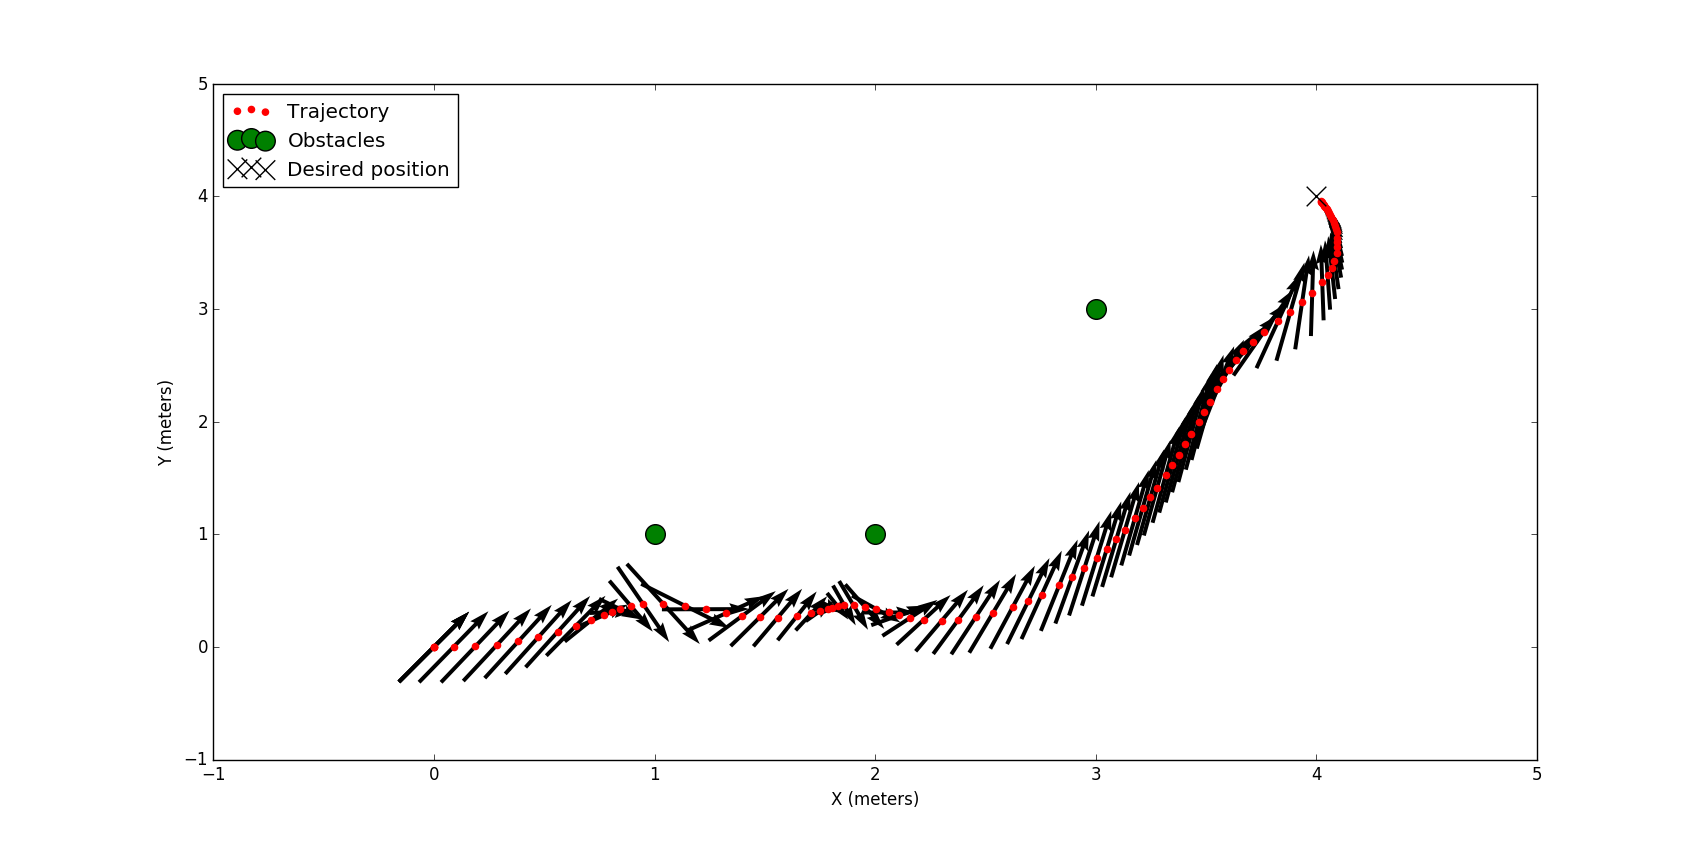
\includegraphics[width = 65mm]{nav_kbki.png}}
%   \caption{Autonomous navigation implemented on Kobuki} \label{f:kbki}
% \end{figure}
\begin{figure}
  \centering
  \subfloat[Attractive force applied to the mobile robot]{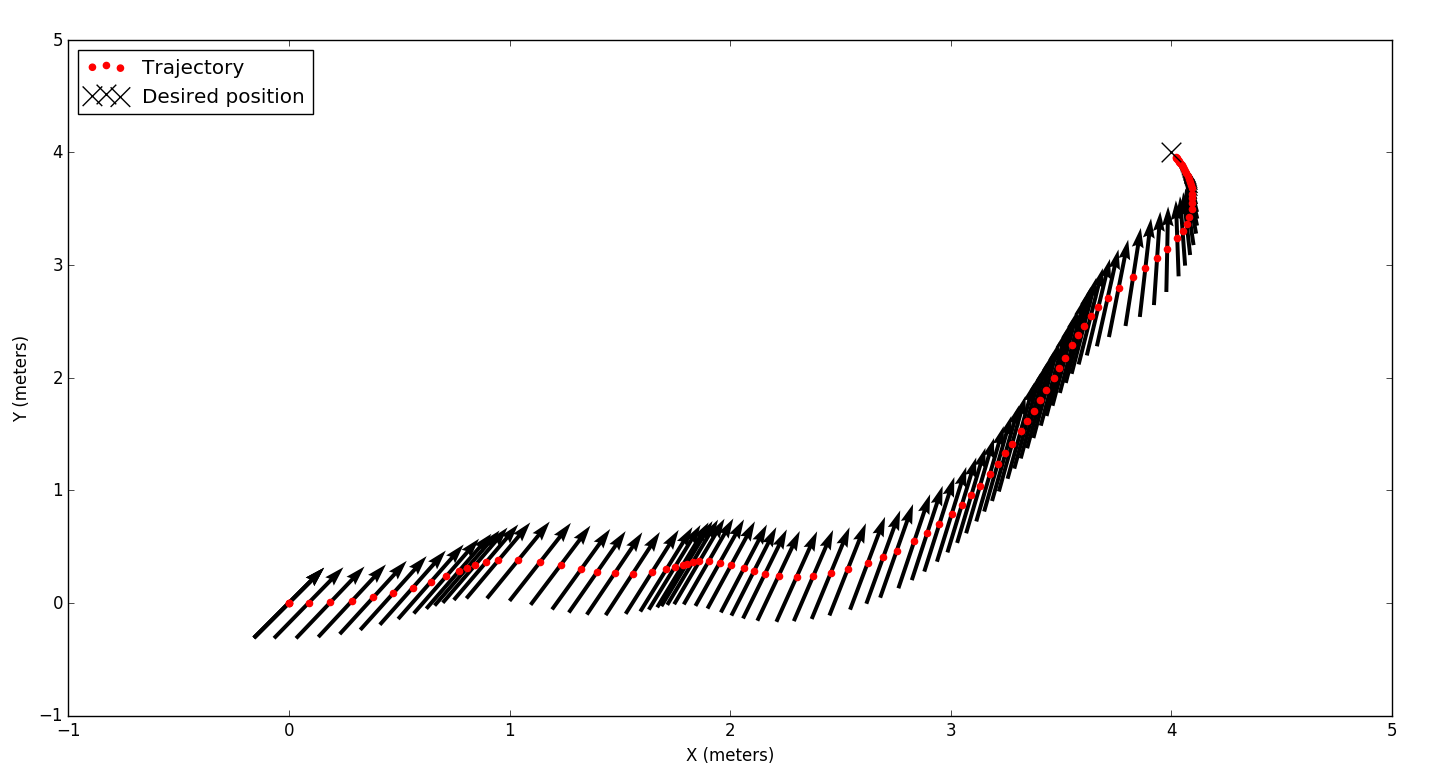
\includegraphics[width = 60mm]{attr_kbki.png}}\\
  \subfloat[Repulsive force applied to the mobile robot] {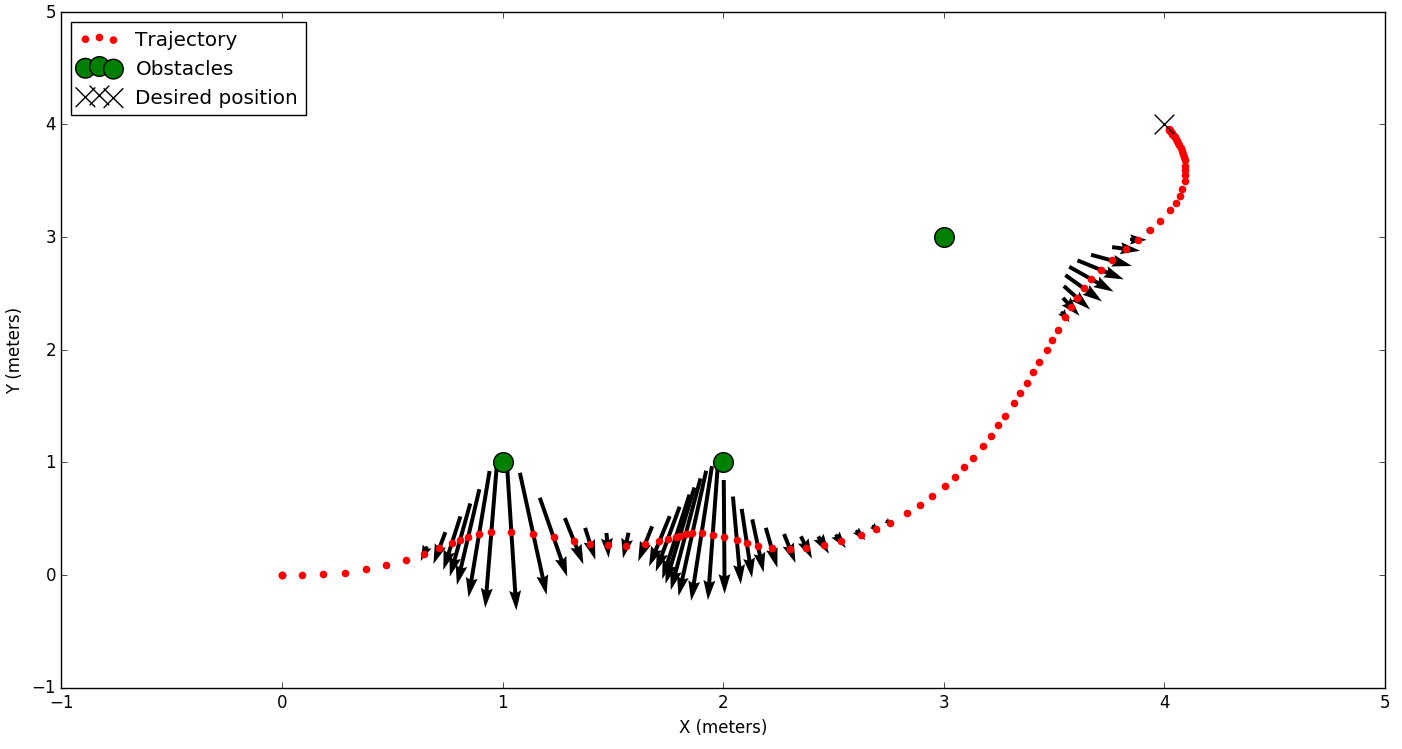
\includegraphics[width = 60mm]{rep_kbki.png}}\\
  \subfloat[Navigation force applied to the mobile robot]{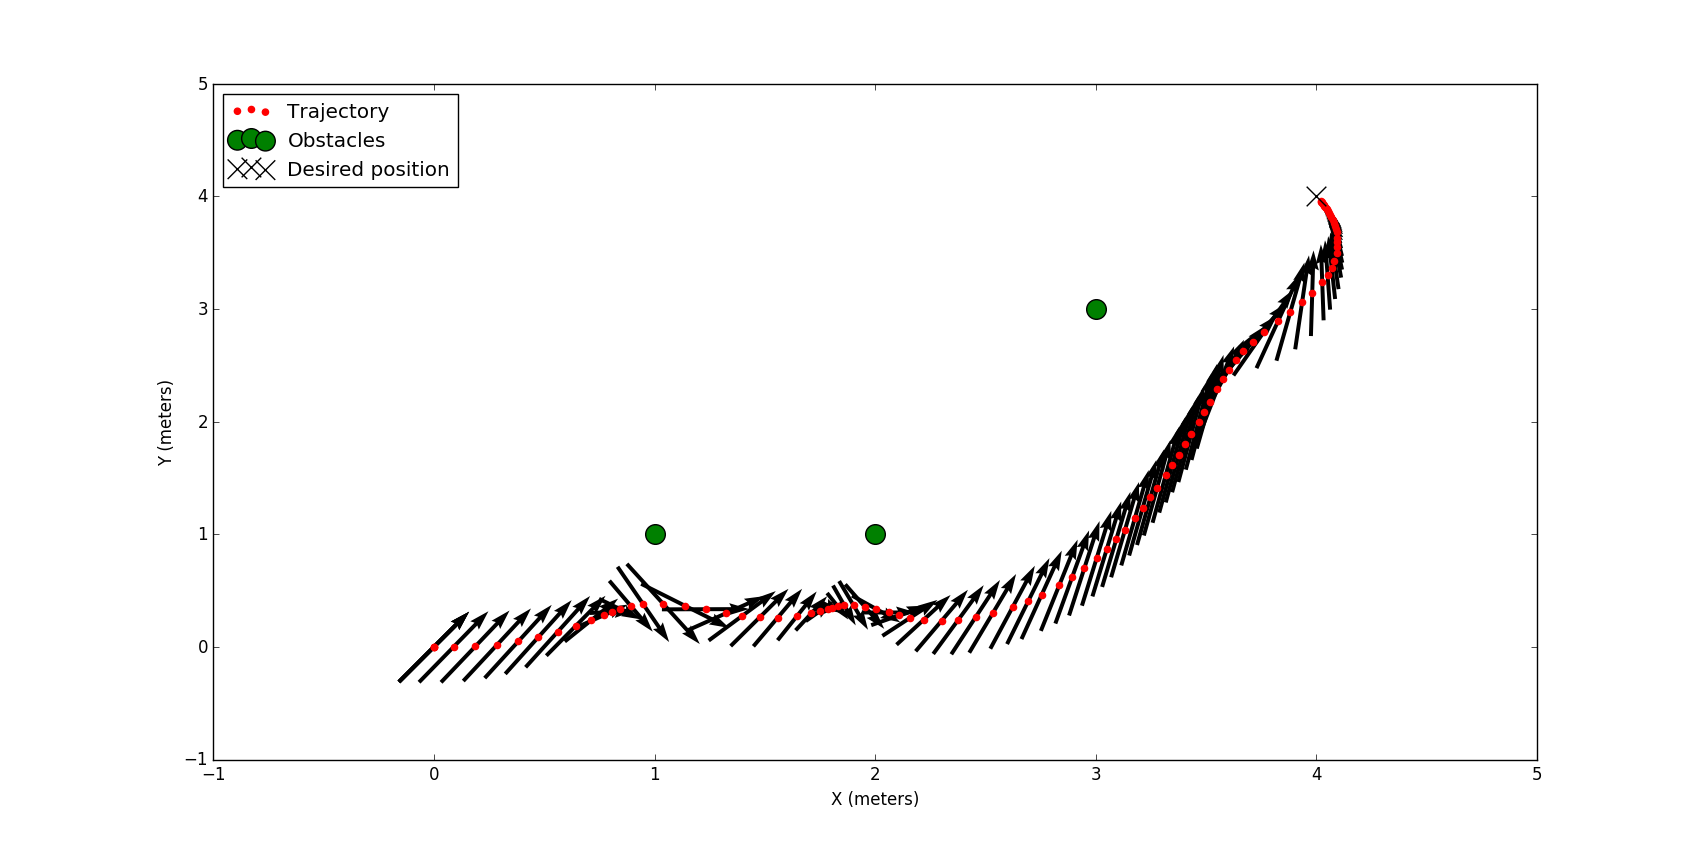
\includegraphics[width = 60mm]{nav_kbki.png}}
  \captionsetup{font=footnotesize}
  \caption{Autonomous navigation implemented on Kobuki} \label{f:kbki}
\end{figure}

\subsection{Autonomous Navigation with Lidar}

To test the whole framwork, we used a lidar (RPLidar A2) which was installed on
top of the kobuki robot. The usage is the continuous update of the obstacles
positions as the robot moves.
% Using ROS, he subscribed to the topic called / scan to
% obtain the measuring ranges of the sensor. With these values, a conversion of
% polar coordinates to Cartesian coordinates was made, in order to know the
% positions of the obstacles within the workspace. Then it was necessary to
% create a message in ROS and also a topic to be able to publish the Cartesian
% coordinates obtained from the 2D map generated by the lidar.  In order for the
% kobuki to be able to move on the map generated by the lidar sensor, the
% reference system of the robot must be taken to the reference system of the
% lidar. Once this is done, the autonomous navigation algorithm is subscribed to
% the coordinates sent by the lidar and thus can generate its own trajectory
% avoiding obstacles.  To perform this test, two boxes were placed in the
% workspace. The position was placed as goal ($ x = 4, y = 0 $).In Figure
% \ref{f:kbki_lidar}(a) you can see the path of the robot in blue and the arrows
% that indicate the force of the robot that bring the robot to the desired
% position. Also, in Figure \ref{f:kbki_lidar}(b) you can see the green dots that
% represent the environment where the kobuki is moving and you can also see the
% arrows that go out avoiding the kobuki can hit the boxes. Finally in Figure
% \ref{f:kbki_lidar}(c) you can see the navigation force that makes the robot can
% move autonomously.
The robot uses ROS topics to get the information of the sensor which is
composed of the range and the orientation of every measured point, as the lidar
rotates. The bearing and range information was then converted to Cartesian
coordinates to know the Cartesian positions of the obstacles within the
workspace, which is the input to the main algorithm. In order for the kobuki to
be able to move within the map generated by the lidar, the reference frame of
the robot was taken as the frame of the lidar. Then, the autonomous navigation
algorithm could use these coordinates of the obstacle to generate its own
trajectory avoiding obstacles. For the whole test, two boxes were placed in the
workspace. The goal position was ($x=4,y=0$). Fig.~\ref{f:kbki_lidar}(a) shows
the path of the robot in blue and the arrows that indicate the force that takes
the robot to the desired position. Fig.~\ref{f:kbki_lidar}(b) shows the full
map, where green dots represent the environment, sensed by the lidar, where the
robot is moving. As observed, these arrows point out of the obstacle providing
autonomy to the robot as it tries to reach the goal. Finally in
Fig.~\ref{f:kbki_lidar}(c) the whole navigation force that drives the motion is
shown.
% \begin{figure}
% 	\centering
% 	%\subfloat [Kobuki with lidar in workspace]{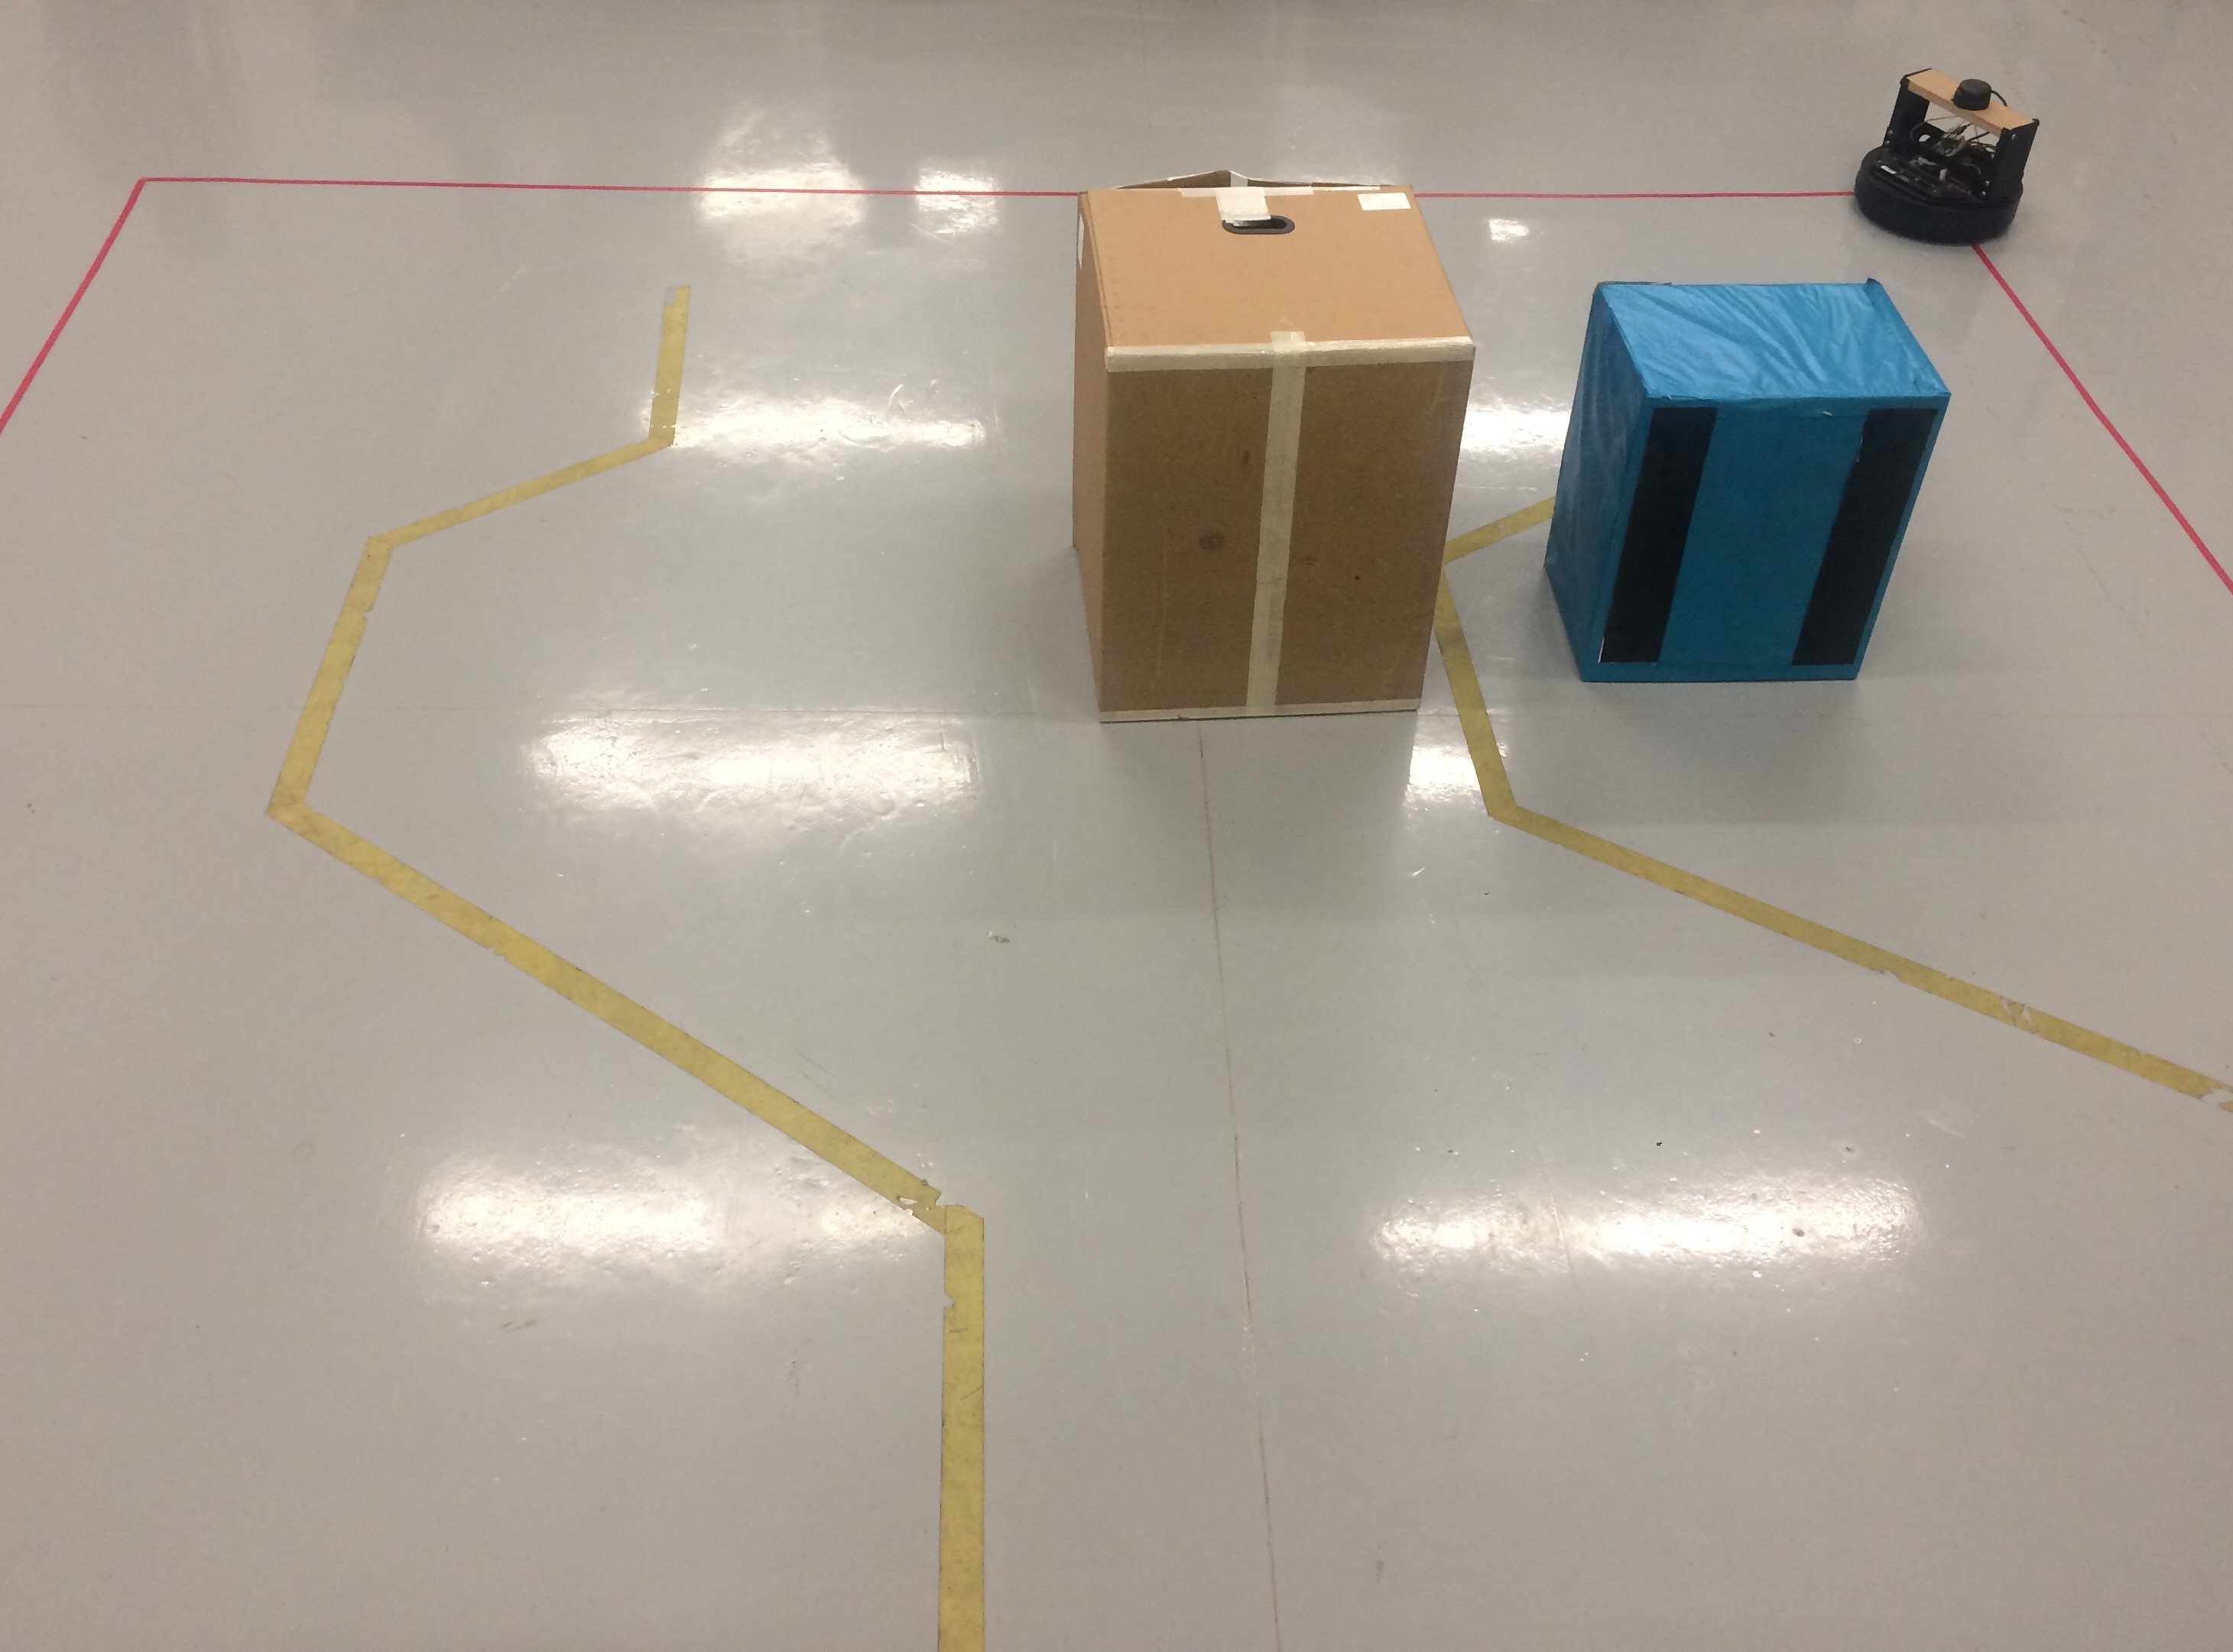
\includegraphics[width = 70mm]{kobuki_201.jpg}}\\
% 	\subfloat[Attractive force applied kobuki with lidar]{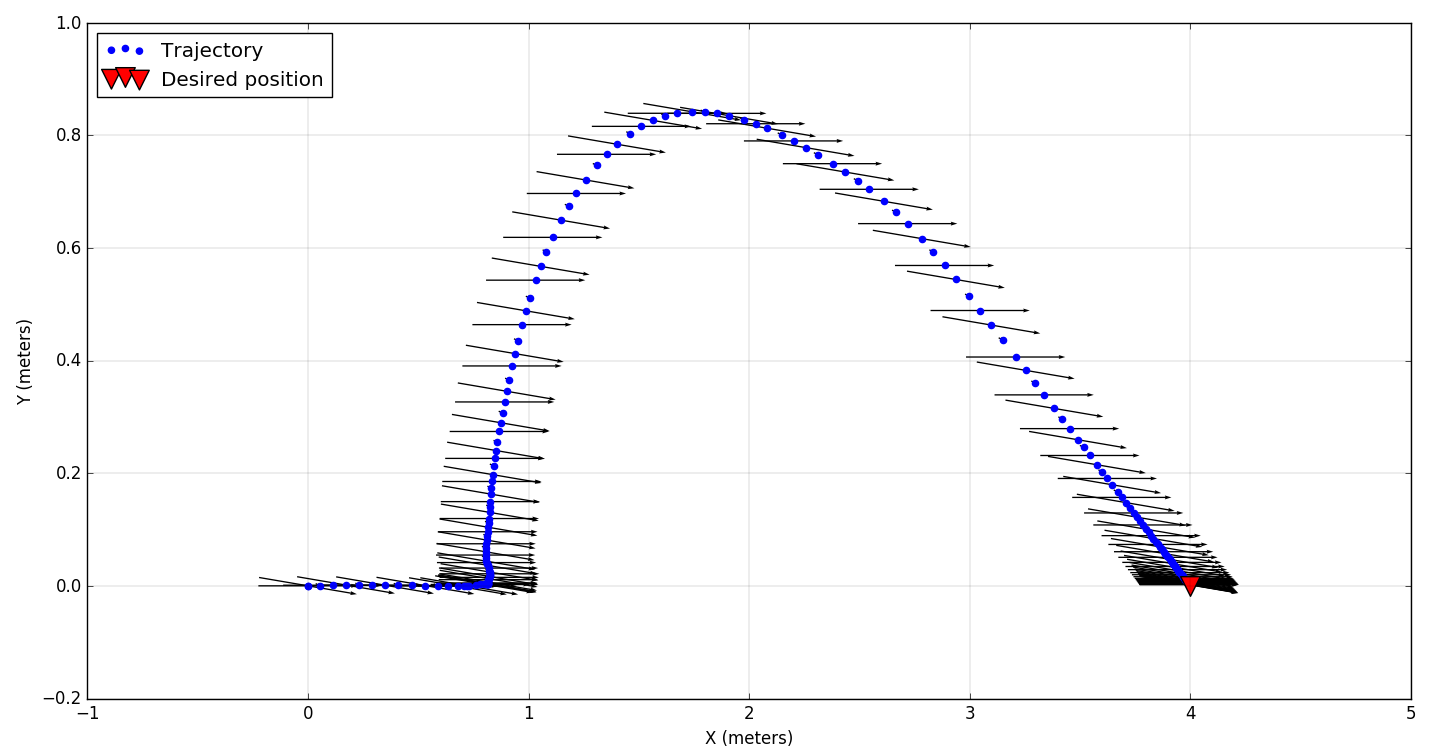
\includegraphics[width = 75mm]{fattr_lidar.png}}\\
% 	\subfloat[Attractive force applied kobuki with lidar]{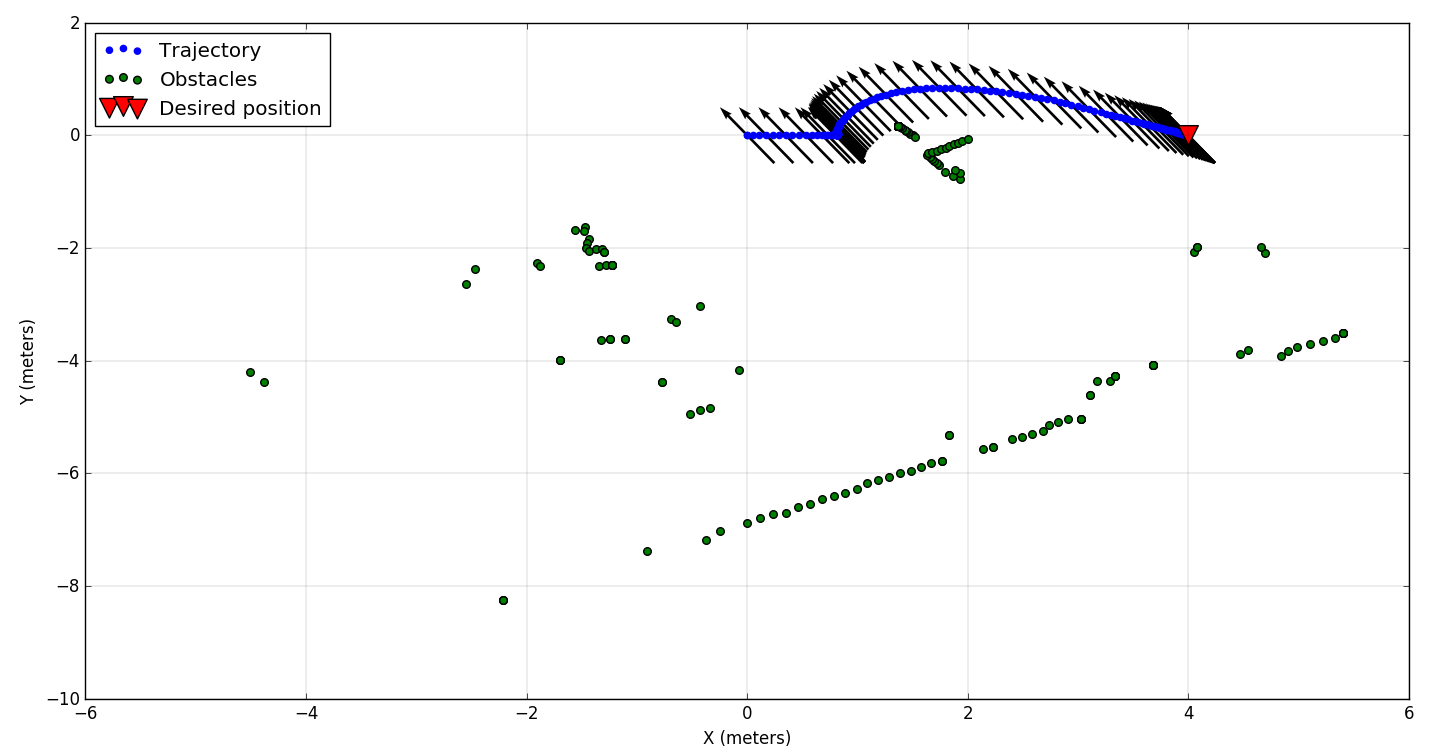
\includegraphics[width = 75mm]{frep_lidar.png}}\\
% 	\subfloat[Attractive force applied kobuki with lidar]{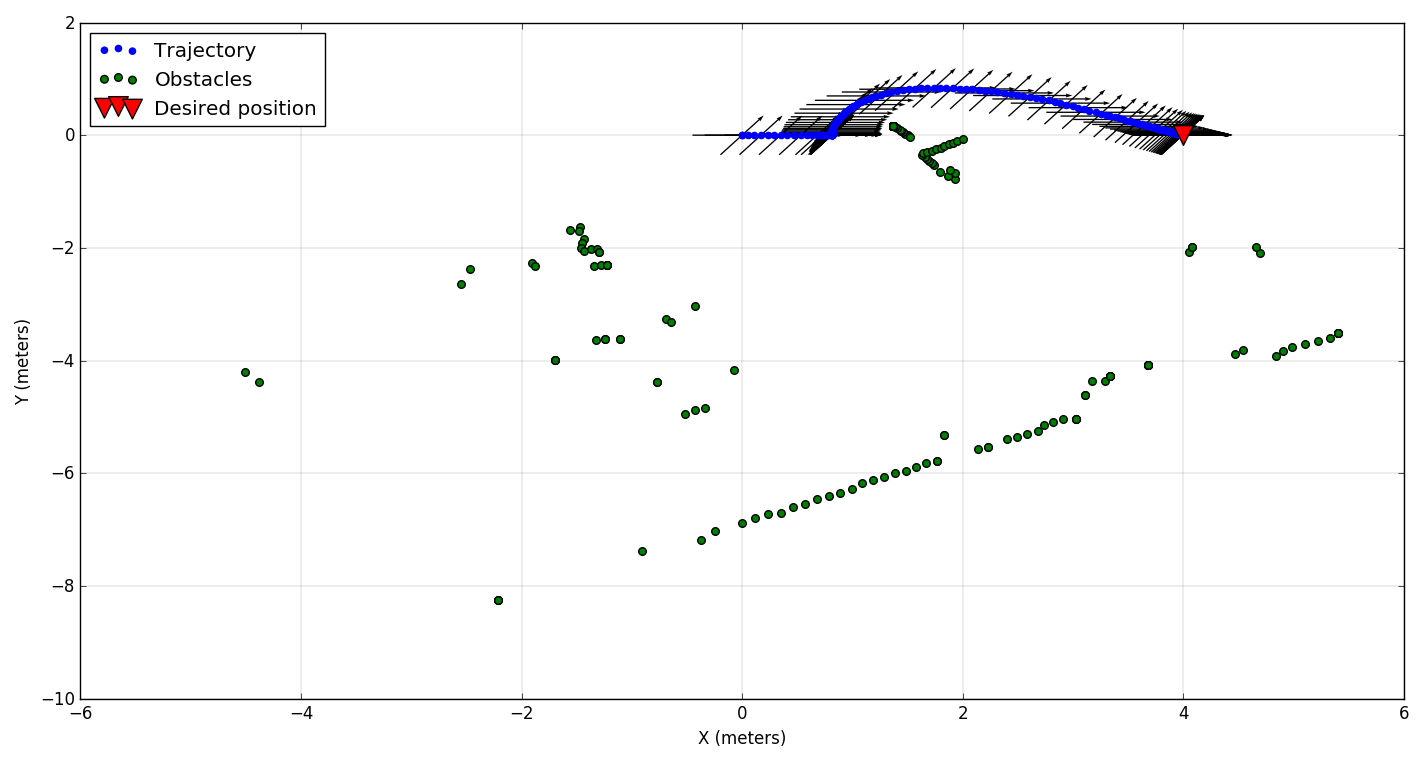
\includegraphics[width = 75mm]{fnav_lidar.png}}\\
% 	\caption{Autonomous navigation with lidar implemented on Kobuki} \label{f:kbki_lidar}
% \end{figure}

\begin{figure}
  \centering
  % \subfloat [Kobuki with lidar in workspace]{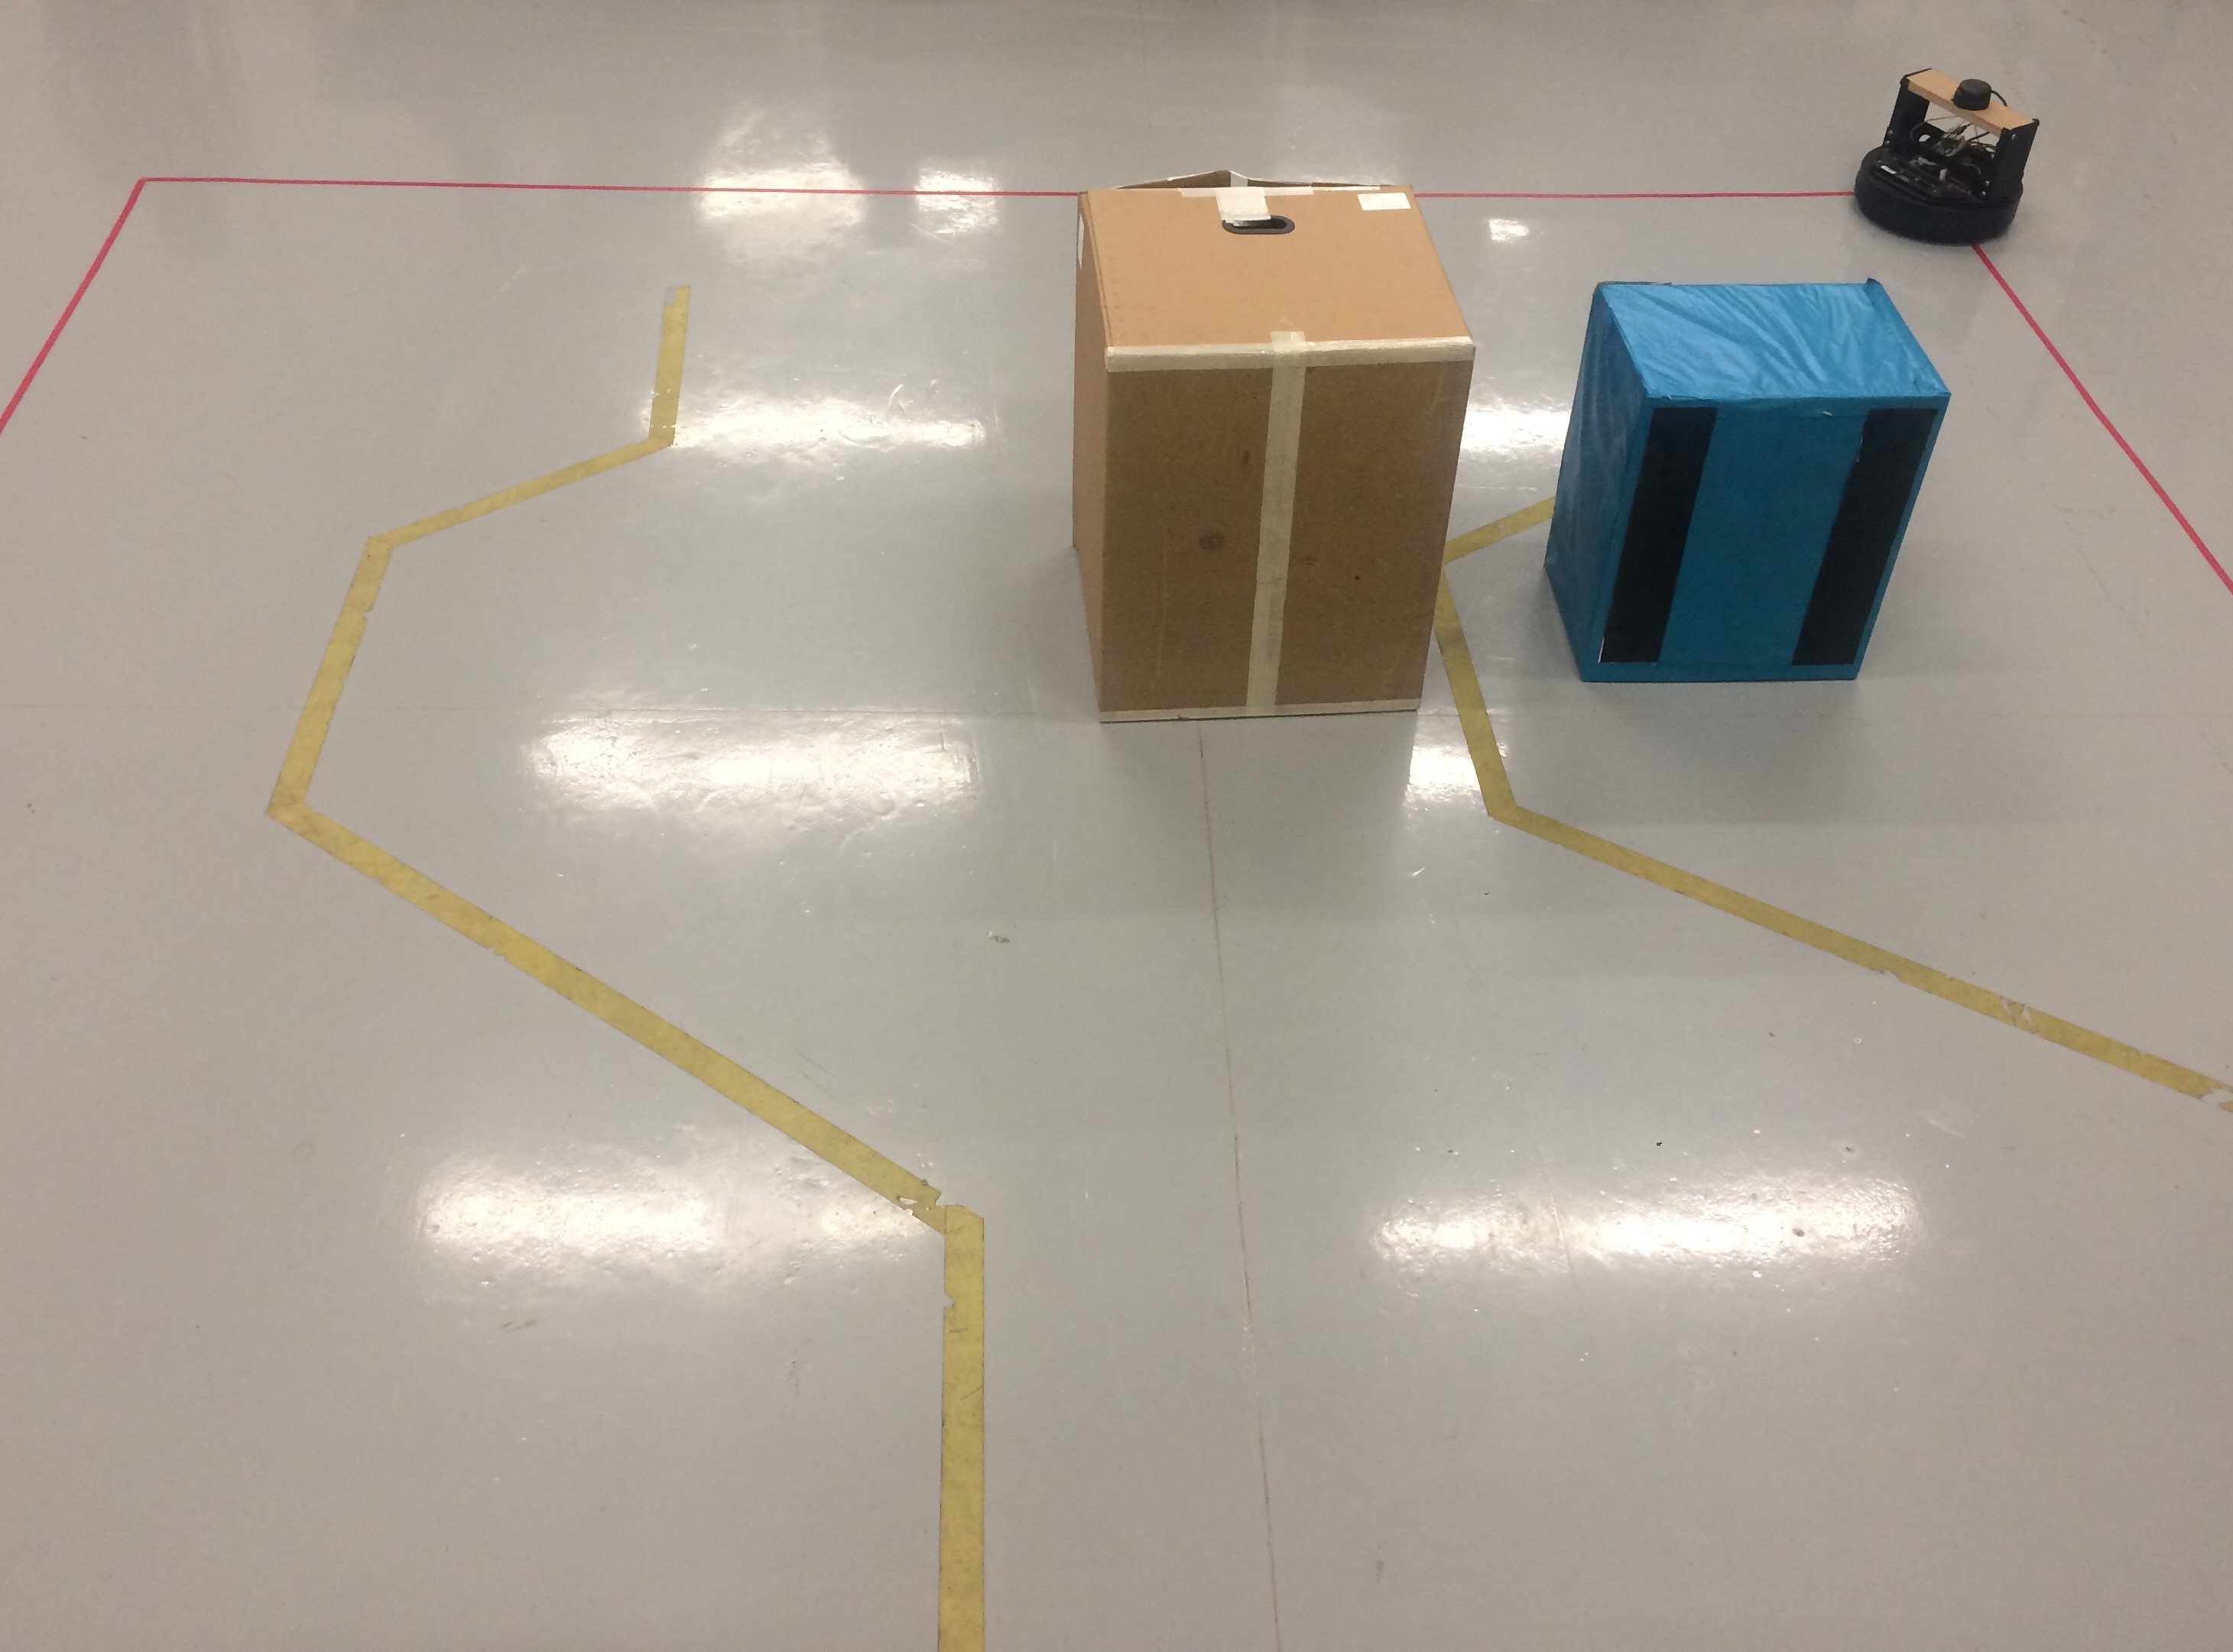
\includegraphics[width = 70mm]{kobuki_201.jpg}}\\
  \subfloat[Online attractive force applied to the robot]{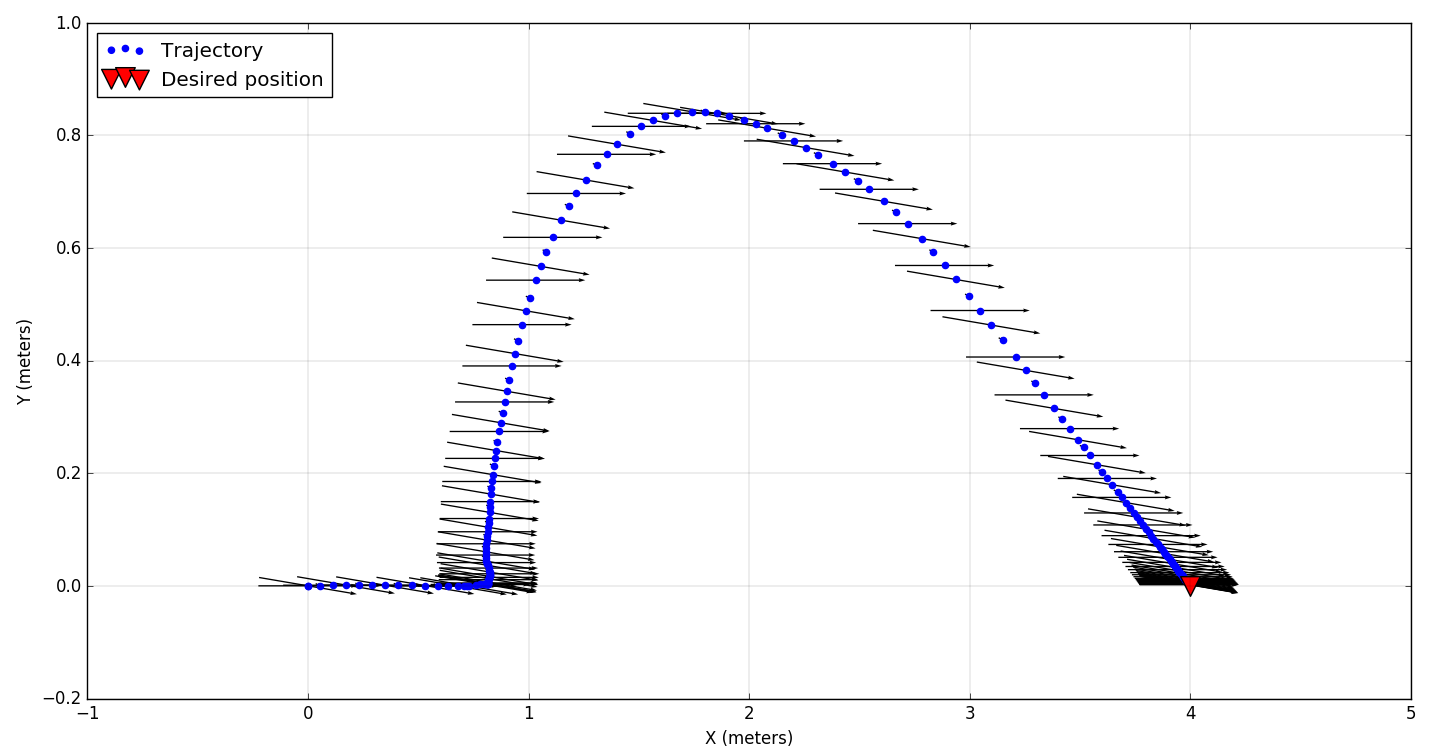
\includegraphics[width = 70mm]{fattr_lidar.png}}\\
  \subfloat[Online repulsive force applied to the robot]{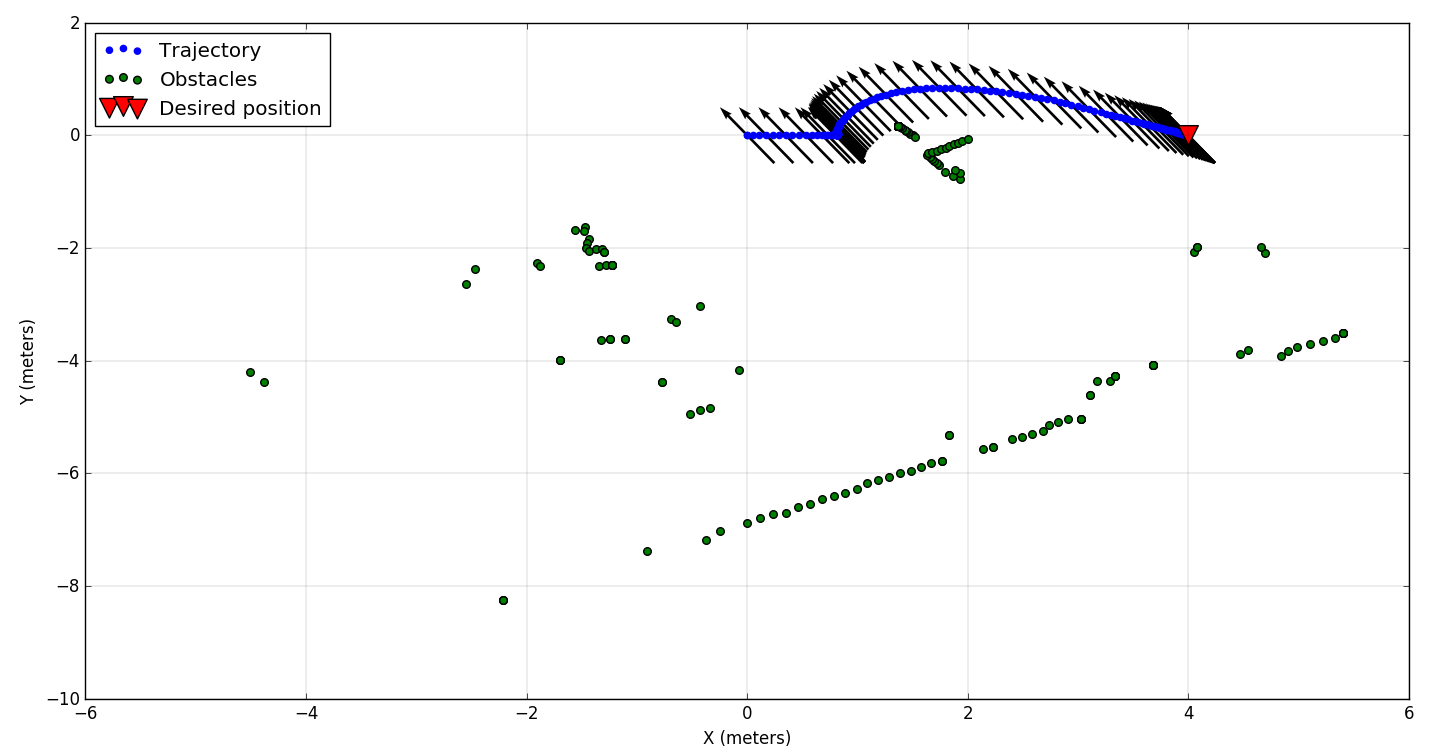
\includegraphics[width = 70mm]{frep_lidar.png}}\\
  \subfloat[Online resulting force]{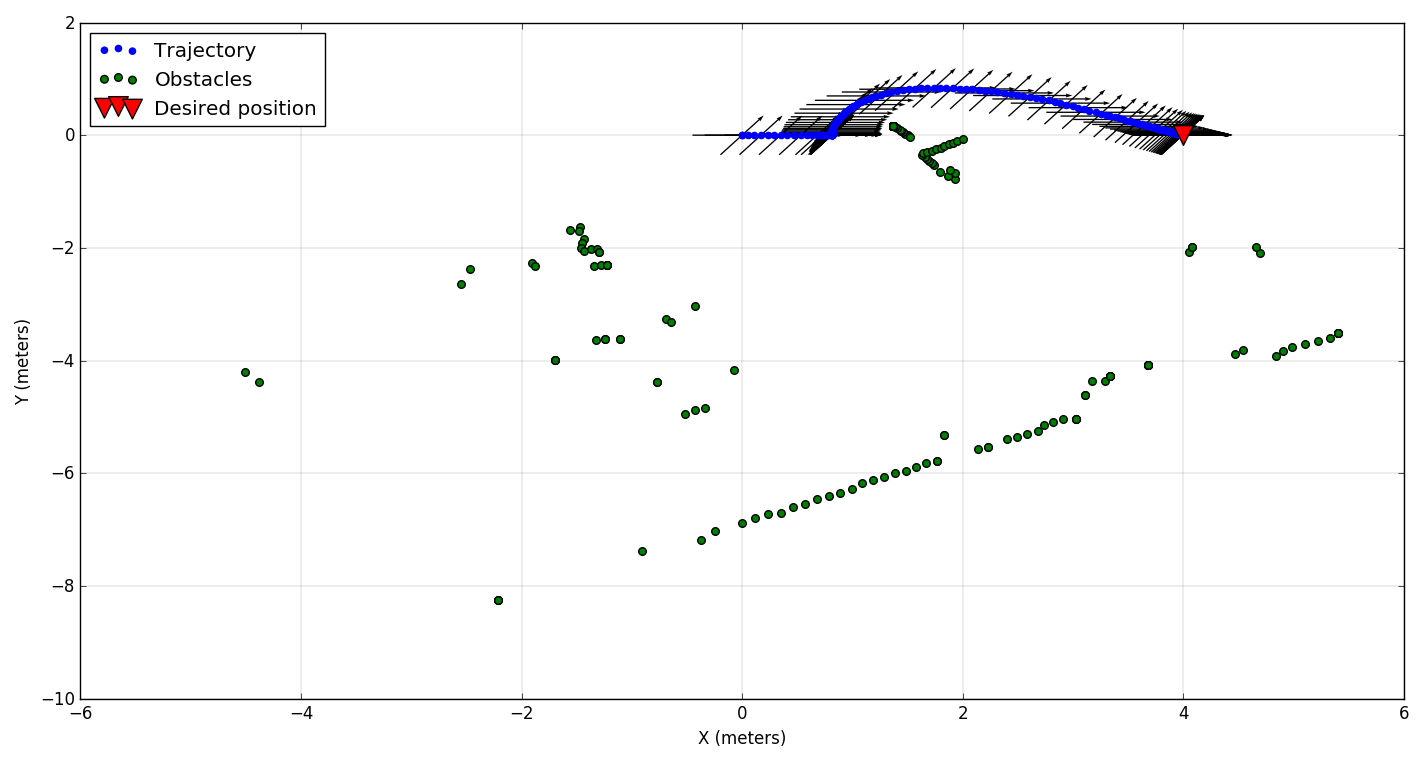
\includegraphics[width = 70mm]{fnav_lidar.png}}\\
  \captionsetup{font=footnotesize}
  \caption{Attractive and repulsive fields, and trajectory that the real robot
    follows using online data coming from the Lidar mounted on top of it} \label{f:kbki_lidar}
\end{figure}

\section{Conclusion}
\label{sec:conclusion}
We presented a whole framework for autonomous motion based on Artificial
Potential Fields and a closed-loop feedback controller. This was applied to
navigation tasks of a differential drive robot. The motion controller is based
on polar coordinates. Results for the motion controller proved to be a solution
to the non-holonomic constraints that the robot presents. In the same way, the
performance of the robot in simulation shows its rapid convergence through
smooth trajectories. Tests on a real Kobuki differential-drive robot show
successful results. They also demonstrate the robot's capability of autonomous
motion despite the unknown configuration of the environment. The lidar provided
information of the environment so that the robot can decide its motion towards
the goal avoiding obstacles in real time.

%We presented a controller based on Artificial Potential Field and a closed-loop feedback controller for navigation tasks of a differential drive robot. The motion controller differs from other works because it bases its frame in polar coordinates. Results for the motion controller proved to be a solution to the non-holonomic constraints that the robot presents. In the same way, the performance of the robot in simulation shows its rapid convergence through smooth trajectories.
% Tests on the Kobuki robot show successful results. It also demonstrates the robot's autonomy despite the unknown configuration of the environment, since only odometry is used. It is demonstrated that by placing the lidar on the Kobuki robot, it can decide its obstacles in real time and can evade them without any problem reaching the goal.
\bibliographystyle{IEEEtran}
\bibliography{biblio.bib}
\end{document}

% Prueba
